% !TeX encoding = ISO-8859-1
% Bachelor Thesis/Master Thesis Template
% based on Disseration Template by J�rn Malzahn:
% Last update: 2014/03/13 jma
% This template has been designed to be compliant with the requirements of the VDI Verlag-
% See VDIVerlag-Hinweise-31_03_2013.pdf for details. The basic principle of these requirements is: you submit a compliant A4 print and they will guarantee a high quality A5 book.
%
%
% NOTE: The template is still under developement.


\documentclass[12pt,a4paper,twoside,headsepline,captions=tableheading,toc=bibliography,openany]{scrbook}

%% For a draft version of your thesis use this line.
%\documentclass[draft,12pt,a4paper,twoside,headsepline,captions=tableheading,toc=bibliography,openany]{scrbook}
%% It uses the draft switch, which will not include the graphics in your output document. Instead it draws bounding boxes for each figure and highlights overfull boxes, and highlights exceeding margins. This is particularly usefull to hunt down overfull boxes.

% useful scripts including if/then/else
\usepackage{etoolbox}

% set language to english, compile two times after changing
\newtoggle{lang_eng}
\settoggle{lang_eng}{true} % true: english, false: german

%Self-defined hyphenations
% !TeX encoding = ISO-8859-1
% Just continue this space separated list
\hyphenation{Tech-ni-sche Uni-ver-si-t�t Dort-mund}

% additional packages
% !TeX encoding = ISO-8859-1
% ################################
% PAGE GEOMETRY
% ################################
%% Use package geometry instead of a4wide!
\usepackage{geometry}	

\geometry{top=25mm,bottom=25mm,left=21mm,right=21mm,headsep=6mm,footskip=11mm,bindingoffset=8mm}

%% Visualization of the page layout
%\usepackage{layouts}
% commands:
%\printinunitsof{cm}
%\currentpage
%\pagedesign

%% Font
% Latex mit deutschen Umlauten:
% http://www.cs.albany.edu/~herrmann/latex_umlaute/

\usepackage[ansinew]{inputenc}
\usepackage[T1]{fontenc}	% EC-Schriften verwenden (vs. DC) da 8-Bit
				% EC-Schriften als T1-kodierten CM-Schriften
				% European/Ext.-Computer-Modern-(EC)-Schriften
				% Umlaute, Anf�hrungszeichen ...
				% => Umlauten koennen richtig getrennt werden
				% FAQ 5.3.2
\usepackage{ae,aecompl}		% virtuelle-CM-Fonts
				% da EC nicht als PostScript-(Type-1) verfuegbar
				% => keine echten Umlaute im PDF-Dokumen 
				%(Problem bei Suche)
				% By loading the ae package (\usepackage{ae}), 
				% you loose some characters as mentioned in 
				% README. 
				% The package aecompl by Denis Roegel restores
				% these characters which are taken from the ec 
				% fonts. If you use pdftex, you will get these 
				% characters as bitmaps, but this might be 
				% better than not having them at all.
\usepackage[sc]{mathpazo} % Palatino (not Palatino Linotype!) as font with serifs
\linespread{1.05}         % Palatino needs more space between lines
\usepackage[scaled=.90]{helvet} % Helvetica as font without serifs
\usepackage{courier} % Courier as type writer font
%% Euro symbol
\usepackage{textcomp} % Euro symbol that fits to Palatino (use \texteuro)

%% Create commands and macros with two optional parameters
\usepackage{twoopt}

%% Customized chapter headings
\usepackage{titlesec}
\titleformat{\chapter}[display]
{\filleft\huge\bfseries\sffamily} % Size of headings and chapter number
{\vspace{-5ex}\fontsize{100pt}{80pt}\selectfont\thechapter}
{-2ex} %  horizontal separation between label and title body 
{\vspace{1ex}} % code preceding the title body
[\vspace{1ex}] % code following the title body


%% Math
\usepackage{amsmath}%
\usepackage{amsfonts}%
\usepackage{amssymb}%
\usepackage{mathtools}%
\usepackage{amsthm}


%% Theorems
\newtheoremstyle{myTheoremStyle}% name
%{2\lineskip}      % Space above
%{2\lineskip}      % Space below
{11pt}      % Space above
{11pt}      % Space below
{\itshape}  % Body font
{}          % Indent amount (empty = no indent, \parindent = para indent)
{\bfseries} % Thm head font
{:}         % Punctuation after thm head
{.5em}      % Space after thm head: " " = normal interword space;{\newline = linebreak}
{}          % Thm head spec (can be left empty, meaning 'normal')
% define theorems in theorems.tex



%% Language settings
\usepackage[\iftoggle{lang_eng}{english}{ngerman}]{babel}
\usepackage[babel,autostyle]{csquotes}


%% Tables
\usepackage{tabularx}
\usepackage{booktabs}

%% for compactitem
\usepackage{paralist}         

%% check whether compiler is set to latex or pdflatex
\usepackage{ifpdf} 

%% Include without pagebreak
\usepackage{newclude} 
% command 
% use \include*{file}

%% Figures
\usepackage{graphicx} % Graphicx-package
\usepackage{subfigure}  % To place figures side by side, if you wish to do that in latex... It is recommended to do that externally.
\usepackage[normal,small]{caption} % Customise the captions in floating environments

% Convert eps to pdf
\ifpdf
	\usepackage{epstopdf}
\fi

\usepackage{psfrag} % To correct the mess Matlab produces in figures!

\usepackage{pgfplots} % include TIKZ support
% TIKZ: Draw vector images directly in matlab or use the matlab exporter plugin:
% Export Matlab-Plots using: matlab2tikz (http://www.mathworks.com/matlabcentral/fileexchange/22022-matlab2tikz)
% Need help?: christoph.roesmann@tu-dortmund.de
%\usepackage{tikz,pgfplots}
\pgfplotsset{compat=newest}
\pgfplotsset{plot coordinates/math parser=false}
\iftoggle{lang_eng}{}
{
\pgfplotsset{/pgf/number format/use comma} % Kommata f�r Dezimaldarstellung
\pgfplotsset{/pgf/number format/.cd,1000 sep={\,}} % Trennzeichen bei 1000
}
\newlength\figureheight
\newlength\figurewidth
\makeatletter
\pgfplotsset{ % Korrektur der Legenden, die unter dem Plot angezeigt werden (legend pos = outer south /outer north)
    every axis x label/.append style={
        alias=current axis xlabel,
    },
    legend pos/outer south/.style={
        /pgfplots/legend style={
            at={%
                (%
                \@ifundefined{pgf@sh@ns@current axis xlabel}%
                {xticklabel cs:0.5}%
                {current axis xlabel.south}%
                )%
            },
            anchor=north,
            legend columns=3,
            font=\small,
            /tikz/every even column/.append style={column sep=10pt, font=\small} %Increase spacing in legend
        }
    },
    legend pos/outer north/.style={
        /pgfplots/legend style={
            at={(\figurewidth/2,\figureheight+0.2cm)},
            draw=none, % ignore box around legend
            anchor=south,
            legend columns=3,
            font=\small,
            /tikz/every even column/.append style={column sep=10pt, font=\small} %Increase spacing in legend
        }
    }
}
\makeatother

% select unique fontsize (small) at the beginning of each tikz picture
\tikzset{every picture/.style={font issue=\small},
         font issue/.style={execute at begin picture={#1\selectfont}}
        }
\tikzset{fontscale/.style = {font=\small}
        }
% add arrow pins to axis by default
\tikzset{every axis/.style={
axis lines = left % middle
}
}  

        
% Externalize tikz image
% Many tikz images or tikz images with lots of data can imply a full latex buffer and therefore stop the comilation.
% If you enable externalization, tikz images are precompiled into an eps/pdf image.
% They are recompiled automatically after updating the tikz image (make sure to use recent Latex Distributions (2014+)) 
% All you need to do is to add an argument (enable-write18 or shell-escape) to the latex executable 
% in order to allow system calls:
% On Windows systems:
% 	 latex.exe [other arguments] -enable-write18 %.tex
% 	 pdflatex.exe [other arguments] -enable-write18 %.tex
% On Unix systems (Mac/Linux):
% 	 latex.exe [other arguments] -shell-escape %.tex
% 	 pdflatex.exe [other arguments] -shell-escape %.tex

\ifnum\pdfshellescape=1
% System calls enabled
	%\usetikzlibrary{external} % not up to date at the moment
	\usepgfplotslibrary{external}
	

	%\ifpdf
   	%%%%%   DEPRECATED. Update pgfplots package (>Sept 2014). 
   	%%%%%				The new version automatically distinguishes between pdflatex and dvips.
	%%%%%				Uncomment only if you still have problems.
	%%%%%				This code will removed in further versions.
	%\else  % only for latex dvi/ps
	%	\tikzset{external/system call={latex \tikzexternalcheckshellescape -halt-on-error
	%	-interaction=batchmode -jobname "\image" "\texsource" && % replace && with ; in TexLive u.a.
	%	dvips -o "\image".ps "\image".dvi  % && ps2eps "\image.ps"
	%	}}
	%\fi

	\tikzexternalize[prefix=Abbildungen/tikz-extern/] % folder to store precompiled tikz images (Make sure, folder already exists!!!)

	% Some packages are not compatible with externalization. Create wrapped code to disable externalization:
	\makeatletter
	\AtBeginDocument{
		% for those using the todonodes package: this command disables the externalization mechanism from the inserted todonotes.
		\@ifpackageloaded{todonotes}{ 
			\renewcommand{\todo}[2][]{\tikzexternaldisable\@todo[#1]{#2}\tikzexternalenable} 
		}{}
		% missing-?gure package:
		\@ifpackageloaded{xmissingfigure}{ 
			\newcommand{\xmissingfigure}[2][]{\tikzexternaldisable\missingfigure[#1]{#2}\tikzexternalenable}
		}{}
	}
	\makeatother
\fi




% By default precompiled tikz images are named in order of appearance. 
% If you use this macro (\includetikz{}), the temporary file will be named similar to the original tikz file. 
%\newcommand{\includetikz}[1]{%
%	 \ifnum\pdfshellescape=1
%    	\tikzsetnextfilename{#1}%
%	 \fi
%    \input{Abbildungen/#1.tikz}%
%}
% This version adds two optional parameters to specify figurewidth and figureheight
\newcommandtwoopt{\includetikz}[3][0.9\linewidth][5cm]{ % optinal parameters [width][height]
	\ifnum\pdfshellescape=1
    	\tikzsetnextfilename{#3}%
    \fi
    \setlength\figurewidth{#1} 
    \setlength\figureheight{#2} 
    \input{Abbildungen/#3.tikz}%
}

% if you are using older latex distributions (<2014), the precompiled tikz images are not updated automatically, therefore run this command to update all images:
%\tikzset{external/force remake} % Recompile all tikz images




%% Colors for text
\usepackage{color}
\usepackage{colortbl}
% Define user colors in RGB
\definecolor{black}{rgb}{0.0,0.0,0.0}
\definecolor{darkgray}{rgb}{0.8,0.8,0.8}
\definecolor{lightgray}{rgb}{0.95,0.95,0.95}
% Example:
%\begin{tabular}{lll>{\columncolor{lightgray}}l}
%\rowcolor{darkgray}
%No. & Supported Feature   & Octet & Bit \\
%0   & Flow Control Mode   & 0     & 0   \\
%\rowcolor{lightgray}
%1   & Retransmission Mode & 0     & 1   \\
%2   & \cellcolor{darkgray}Bi-directional QoS  & 0     & 2   \\
%31  & Reserved for feature mask ext. & 3 & 7
%\end{tabular}

%% Rotate figures
\usepackage{rotating}
\usepackage{import}

%% Nomenclature
\usepackage[noprefix,intoc,\iftoggle{lang_eng}{english}{german}]{nomencl}
\setlength{\nomlabelwidth}{.25\hsize}
\setlength{\nomitemsep}{-\parsep}
% Split nomenclature for symbols and abbreviations
\renewcommand{\nomgroup}[1]{%
\ifstrequal{#1}{C}{\vspace{3mm}\item[\textbf{\iftoggle{lang_eng}{Roman symbols}{Lateinische Symbole}}]}{
\ifstrequal{#1}{B}{\vspace{3mm}\item[\textbf{\iftoggle{lang_eng}{Greek symbols}{Griechische Symbole}}]}}{
\ifstrequal{#1}{A}{\vspace{3mm}\item[\textbf{\iftoggle{lang_eng}{Abbreviations and acronyms}{Abk�rzungen und Akronyme}}]}{}}} 



\makenomenclature %Generates a %tm.nlo file
% Postprocessor settings: run makeindex.exe  with argument list: %tm.nlo -s nomencl.ist -o %tm.nls (TeXnicCenter -> Ausgabeprofile)
% Use \printnomenclature to create a nomenclature in your document
% Use \nomenclature[A]{abrev.}{description} for abbreviations
% Use \nomenclature[1symbol]{symbol}{description} for greek symbols
% Use \nomenclature[3symbol]{\symbol}{description} for greek symbols. Note: Rewriting the symbol name without the backslash is important for correct alpha numeric ordering! This is particularly visible if you have hats, tilde, dots, bars or anything like that to modify your greek letter.
%
% TexStudio:
% 1. Step: configure Makeindex 
%  Compile flags: Makeindex: makeindex.exe %.nlo -s nomencl.ist -o %.nls 
% 2. Step: run Makeindex during compilation
%  TexStudio: Tab Create: Default compiler: add makeindex (click on screwdriver button)
%
% For additional information see:
% http://www.ctan.org/tex-archive/macros/latex/contrib/nomencl/


%% Bibliography using Biblatex
% Simple bibtex is outdated. Biblatex provides a whole lot of nice features.
\usepackage[babel=hyphen,style=authoryear-comp,firstinits=true,uniquename=init,isbn=false,dashed=false,backend=bibtex,maxnames=3,minnames=1,maxbibnames=99]{biblatex}
% Detailed information: ftp://ftp.mpi-sb.mpg.de/pub/tex/mirror/ftp.dante.de/pub/tex/macros/latex/contrib/biblatex/doc/biblatex.pdf
%
% Options used here:
% - babel=hyphen -> hyphenation in multiple languages within bibliography. Just add a new field to your bibtex entry to indicate which language to use. Example: hypenation={ngerman} for german hyphenation in english documents, hypenation={english} for english hyphenation in german documents.
% - style=numeric together with defernumbers = true: Citations using reference numbers (e.g. [12] ); defernumbers enables unique reference numbers even with multiple bibliographies
% - backend=bibtex: Avoids the installation of biber

% Increase spacing between two bib items
\setlength{\bibitemsep}{0.5\baselineskip}

\addbibresource{thesis.bib} % Bibtex file 
% Settings for bibliography with external references
%\defbibheading{ref}[References]{
%\pagestyle{myheadings}%
%\markboth{#1}{#1}%
%\section*{#1}%
%}
%\defbibnote{ref}{Parts of the material presented in this work has been originally published in conferences and journals. These publications as well as the resources by other researchers are summarized in the following list:}

% Settings for the bibliography with supervised theses
%\DeclareBibliographyCategory{thes}	 
%\defbibheading{thes}[Supervised theses]{
%\newpage
%\pagestyle{myheadings}%
%\markboth{#1}{#1}%
%\section*{#1}%
%}
%\defbibnote{thes}{A number of ideas grown during this work emerged from discussions in the context of supervised theses. Source code and measurement data contributed to the material presented in this work. The contributing theses are:}

% Settings for the bibliography with your published media
%\DeclareBibliographyCategory{media}
%\defbibheading{media}[Published Software and Media]{
%\newpage
%\pagestyle{myheadings}%
%\markboth{#1}{#1}%
%\section*{#1}%
%}
%\defbibnote{media}{During preparation of this work the following media and sources have been published online under open licenses:}

\ifnum\pdfshellescape=1
	\tikzifexternalizing{% fix compatibility problems with defernumbers of biblatex
	        \ExecuteBibliographyOptions{defernumbers=false}
	}{}
\fi

% Make bold labels in bibliography!
% From:  http://tex.stackexchange.com/questions/91570/bibliography-with-biblatex-how-to-achieve-bold-labels-using-the-authoryear-styl
\usepackage{xpatch}
%\xpretobibmacro{author}{\mkbibbold\bgroup}{}{}
%\xapptobibmacro{author}{\egroup}{}{}
%\xpretobibmacro{bbx:editor}{\mkbibbold\bgroup}{}{}
%\xapptobibmacro{bbx:editor}{\egroup}{}{}
%\renewcommand*{\labelnamepunct}{\mkbibbold{\addcolon\space}}

\usepackage{bibspacing}
% Spacing between references. This package requires the file bibspacing.sty
\setlength{\bibspacing}{\baselineskip}

% Conditionally build comments and contents
\usepackage{comment} 
%In preamble:
%% Variant I: Summary only: 
%%\includecomment{summary} %Build latex code within summary environment
%%\excludecomment{content} %Do not build latex code within the content envrionment
%% Variante II: Nur Inhalt:
%%\excludecomment{summary} %Do not build latex code within the summary environment
%%\includecomment{content} %Build latex code within content envrionment
%% Variante III: Summary + Inhalt:
%\includecomment{summary} %Build latex code within summary environment
%\includecomment{content} %Build latex code within content envrionment
%
% Usage in the body. Example:
%\begin{summary}
%\rule{\textwidth}{1pt} % <- visual separation between summary and contents in compiled document
%SUMMARY GOES HERE\\
%\rule{\textwidth}{1pt} % <- visual separation between summary and contents in compiled document
%\end{summary}
%\begin{content}
%This is the content\\
%\end{content}

%% Hyperlinks, has to be the last package!
%\usepackage[colorlinks=true,urlcolor=blue,citecolor=blue,linkcolor=black]{hyperref} % sch�n f�rs PDF
\usepackage[colorlinks=false]{hyperref} % sch�n f�r Druck
\ifpdf
\else
\usepackage[anythingbreaks]{breakurl} % only for ps/dvi
\fi
\color{black} % Make sure the whole text black!


% Path to the graphics/figures
\graphicspath{{./Abbildungen/}} 

%% To keep the overview, create a commented structure or obtain a ready to print version of your work:
% Variant I: Summary only: 
%\includecomment{summary} %Build latex code within summary environment
%\excludecomment{content} %Do not build latex code within the content envrionment
%% Variante II: Nur Inhalt:
%\excludecomment{summary} %Do not build latex code within the summary environment
%\includecomment{content} %Build latex code within content envrionment
%% Variante III: Summary + Inhalt:
\includecomment{summary} %Build latex code within summary environment
\includecomment{content} %Build latex code within content envrionment

% ##########################################################################
% BODY
% ##########################################################################
\begin{document}
%% Uncomment the following three lines to display the page layout. In that case also uncomment line 10 in packages.tex!
%\printinunitsof{cm}
%\currentpage
%\pagedesign

% ##########################################################################
% PREFACE AND INDEXES
% ##########################################################################
% Self-defined environments 
% !TeX encoding = windows-1252
\theoremstyle{myTheoremStyle}

\newtheorem{acknowledgement}{\iftoggle{lang_eng}{Acknowledgement}{Danksagung}}
\newtheorem{algorithm}{\iftoggle{lang_eng}{Algorithm}{Algorithmus}}[section]
\newtheorem{assumption}{\iftoggle{lang_eng}{Assumption}{Annahme}}[section]
\newtheorem{assumptions}{\iftoggle{lang_eng}{Assumptions}{Annahmen}}[section]
\newtheorem{axiom}{Axiom}[section]
\newtheorem{case}{\iftoggle{lang_eng}{Case}{Fall}}[section]
\newtheorem{claim}{\iftoggle{lang_eng}{Claim}{Forderung}}[section]
\newtheorem{conclusion}{\iftoggle{lang_eng}{Conclusion}{Schlussfolgerung}}[section]
\newtheorem{condition}{\iftoggle{lang_eng}{Condition}{Bedingung}}[section]
\newtheorem{conjecture}{\iftoggle{lang_eng}{Conjecture}{Vermutung}}[section]
\newtheorem{convention}{\iftoggle{lang_eng}{Convention}{Konvention}}[section]
\newtheorem{corollary}{\iftoggle{lang_eng}{Corollary}{Korollar}}[section]
\newtheorem{criterion}{\iftoggle{lang_eng}{Criterion}{Kriterium}}[section]
\newtheorem{definition}{Definition}[section]
\newtheorem{example}{\iftoggle{lang_eng}{Example}{Beispiel}}[section]
\newtheorem{exercise}{\iftoggle{lang_eng}{Exercise}{Aufgabe}}[section]
\newtheorem{lemma}{Lemma}[section]
\newtheorem{notation}{\iftoggle{lang_eng}{Notation}{Bezeichnung}}[section]
\newtheorem{problem}{Problem}[section]
\newtheorem{proposition}{\iftoggle{lang_eng}{Proposition}{Satz}}[section]
\newtheorem{remark}{\iftoggle{lang_eng}{Remark}{Bemerkung}}[section]
\newtheorem{solution}{\iftoggle{lang_eng}{Solution}{L�sung}}[section]
\newtheorem{theorem}{Theorem}[section]
\numberwithin{equation}{section}
%-----------------------------------------------------------
% Page numbering for title, abstract, dedication and acknowledgements
% Table of contents has roman page numbering. See VDIVerlag-Hinweise-31_03_2013.pdf for details.
\pagenumbering{roman}
\pagestyle{empty} 

%% Title page
\iftoggle{lang_eng}
	{\makeatletter  % Do not delete this line



\title{
\begin{table}[t]
	\begin{tabular}{p{0.775\columnwidth} r} % 0.775 was 0.85 -> needs a proper fix!
	%  \includegraphics[width=9cm]{tudo} & \includegraphics[width=2.5cm]{rst} \\
		
\includegraphics[width=9cm]{tud_logo_rgb} & 
\includegraphics[width=2.5cm]{rst_rgb}
	\end{tabular}
\end{table}
\LARGE Adapting pre-trained convolutional neural network models for traffic scene labeling\\ 
\vspace{2cm}
{\normalfont\large{{\textbf{Master Thesis}}}\\ 
\vspace{1cm}
\normalfont{submitted to}\\
\vspace{1cm}
\normalfont{Institute of Control Theory and Systems Engineering}\\
\vspace{0.5cm} 
%\normalfont{der}\\
\normalfont{Faculty of  Electrical Engineering and Information Technology}\\ 
%\normalfont{der}\\
\vspace{0.5cm} 
\normalfont{Technische Universit�t Dortmund}\\
\vspace{1cm}
\normalfont{by}\\ 
\vspace{-1cm}
}}
\author{\normalsize{\normalfont{ Carlos Miguel Trevino Campa }}\\ 
\normalsize{\normalfont{Dortmund, Germany}}}
\date{\vspace{2cm}
\raggedright{
\normalsize{\normalfont{Date of Submission: \today }\\ 
\vspace{0.5cm}
\normalfont{\textit{Responsible Professor}: }\\
\normalfont{Univ.-Prof. Dr.-Ing. Prof. h.c. Dr. h.c. Torsten Bertram}\\
\vspace{0.25cm}
\normalfont{\textit{Academic Supervisors}:}\\ 
\normalfont{apl. Prof. Dr. rer. nat. F. Hoffmann}\\
\normalfont{Malte Oeljeklaus, M.Sc.}\\
}}
}

\makeatother  % Do not delete this line
}
	{\makeatletter  % Do not delete this line



\title{
\begin{table}[t]
	\begin{tabular}{p{0.775\columnwidth} r} % 0.775 was 0.85 -> needs a proper fix!
	%  \includegraphics[width=9cm]{tudo} & \includegraphics[width=2.5cm]{rst} \\
		
\includegraphics[width=9cm]{tud_logo_rgb} & 
\includegraphics[width=2.5cm]{rst_rgb}
	\end{tabular}
\end{table}
\LARGE Titel meiner Abschlussarbeit\\ 
\vspace{0.5cm}
\large{Untertitel (optional) }\\
\vspace{2cm}
{\normalfont\large{{\textbf{Masterarbeit / Bachelorarbeit}}}\\ 
\vspace{1cm}
\normalfont{eingereicht am}\\
\vspace{1cm}
\normalfont{Lehrstuhl f�r Regelungssystemtechnik}\\
\vspace{0.5cm} 
%\normalfont{der}\\
\normalfont{Fakult�t f�r Elektrotechnik und Informationstechnik}\\ 
%\normalfont{der}\\
\vspace{0.5cm} 
\normalfont{Technische Universit�t Dortmund}\\
\vspace{1cm}
\normalfont{von}\\ 
\vspace{-1cm}
}}
\author{\normalsize{\normalfont{ Jane Doe }}\\ 
\normalsize{\normalfont{Geburtsort, Geburtsland}}}
\date{\vspace{2cm}
\raggedright{
\normalsize{\normalfont{Abgabedatum: \today }\\ 
\vspace{0.5cm}
\normalfont{\textit{Verantwortlicher Hochschullehrer}: }\\
\normalfont{Univ.-Prof. Dr.-Ing. Prof. h.c. Dr. h.c. Torsten Bertram}\\
\vspace{0.25cm}
\normalfont{\textit{Wissenschaftliche Betreuer}:}\\ 
\normalfont{Dipl.-Ing. Max Mustermann}\\
\normalfont{Dipl.-Ing. Lisa M�ller}\\
}}
}

\makeatother  % Do not delete this line
}
\maketitle

%% dedication
% !TeX encoding = ISO-8859-1
\thispagestyle{empty}
\vspace*{\fill}
\begin{center}
\begin{quote}
"\textit{Das ist die Widmung (optional)}"
\end{quote}
\end{center}
\vspace*{\fill}


%% acknowledgement
% !TeX encoding = ISO-8859-1
\chapter*{\iftoggle{lang_eng}{Acknowledgement}{Danksagung}}
I would like to take this opportunity to express my gratitude to M.Sc. Malte Oeljeklaus
and apl. Prof. Dr. rer. nat. Frank Hoffmann for their guidance and help provided during
the work.

I also express my gratitude to my family and close friends for their constant support during the program.


%% abstract
% !TeX encoding = ISO-8859-1
\chapter*{\iftoggle{lang_eng}{Abstract}{Kurzfassung}}
Modern driver assistance systems aim to automate the task of driving a vehi-cle in increasingly complex situations. In order to handle these situations, a profound understanding of the scene surrounding the vehicle is essential. The rich level of detail found in camera images makes them a natural choice to approach this problem. In computer vision, scene labeling is known as la-beling each pixel in an image with the category of the object or region it belongs to. Existing methods rely on learning databased models from recorded and hand-labeled datasets using machine learning techniques. One method are so called convolutional neural network (CNN) models, which are variants of regular neural networks consisting of a number of convolutional and subsam-pling layers optionally followed by fully connected layers. CNN models de-pict the state of the art in several computer vision problems. However, they typically require large datasets and long computation times during the training phase.
One way to overcome this drawback is to use pre-trained, readily para-metrized models as an initialization and adapt (fine-tune) them to solve a specific problem. For this, the thesis task is to analyze, how existing pre-trained CNN models can be adapted towards the problem of traffic scene la-beling. Therefor the method of fully convolutional networks is to be exam-ined, which does not require complex pre- or post-processing steps and al-lows for adapting CNN models trained for whole-image classification towards scene labeling tasks. The task includes preparing an appropriate dataset for traffic scenes using typical category labels including road, car and pedes-trian.

  
% ##########################################################################
% MAIN CONTENTS
% ##########################################################################
% There is no list of figrues and list of tables in the template. See VDIVerlag-Hinweise-31_03_2013.pdf for details.
\setcounter{page}{1}
\pagestyle{headings} 
\tableofcontents
\newpage

%% nomenclature
% !TeX encoding = ISO-8859-1
%%%%%%%%%%%%%%%%%%%%%%%%%%%%%%%% Nomenclature %%%%%%%%%%%%%%%%%%%%%%%%%%%%%%%%%%%
%See: http://blog.stefan-macke.com/2006/05/03/abkurzungsverzeichnis-mit-latex/

% Page style
\markboth{\nomname}{\nomname}% maybe with \MakeUppercase
\iftoggle{lang_eng}{}{\renewcommand{\nomname}{Nomenklatur}} % use german name


\printnomenclature % There is a bug TeXnicCenter version 2.0 Beta 1. As soon as this line is added to the document the structure pane indicates a missing paragraph. Nevertheless the nomenclature package works correctly. 

%% General variables
\nomenclature{$\mathbf{x}(t)$}{Zustandsvektor zum Zeitpunkt $t$}%
\nomenclature{$u(t)$}{Eingangssignal zum Zeitpunkt $t$}%
\nomenclature{$t$}{Zeit}
\nomenclature{$x,y,z$}{Spatial coordinates}

%% Abk�rzungen
\nomenclature[A]{Abrev.}{Abbreviation}
\nomenclature[A]{KF}{\textbf{K}alman \textbf{F}ilter}

\nomenclature[B]{$\alpha$}{Griechischer Buchstabe}


\cleardoublepage % fixes confused odd/even page order

%% Page numbering in the main part
\pagenumbering{arabic}
\pagestyle{headings} 

% #######################################################
% !TeX encoding = ISO-8859-1
\chapter{Introduction}
\label{ch:Introduction}

\section{Motivation}
\label{sec:Motivation}

Computer vision systems and their capabilities have advanced in the recent years. They make use of the more powerful computer processing capabilities and new learning methods/algorithms to improve the overall performance. Autonomous driving is one of several application that benefits from these advances.
 
In order to obtain a deeper understanding of the surrounding environment, autonomous driving applications can take advantage of camera images. Complex situations can take place in traffic environments, therefore an efficient analysis of the provided images is required. In order to extract the important information contained in the images, different technologies are used (e.g object detection, semantic segmentation, etc). \textit{Semantic segmentation} (pixel classification) simplifies an image by associating a predefined class labels to each pixel, while \textit{Object detection} localizes objects which belong to determined classes. 
 
The purpose of this work is to yield a Semantic segmentation of traffic scenes with an outstanding performance and able to be implemented in real time applications. The selected approach exploits the recent developments in machine learning and more specifically makes use of \textit{Convolutional Neural Networks} (CNNs) using \textbf{Caffe} (\textcite{jia2014caffe}) as framework.

Convolutional Neural Networks (CNNs) have become the mainstream of high-level vision research. They are powerful visual models that yield hierarchies of features, and were successfully used for the first time to solve document recognition (\textcite{lecun1998gradient}). CNNs currently show state of the art performance in high level vision tasks (e.g. image classification, object recognition,object detection, etc.). More information about the success of CNNs is presented in Section ~\ref{sec:pixsemseg}. 

The spatial relation yield in the image semantic segmentation is also benefited from a temporal relation within the continuous stream of images. The previous frames provide information which allows to enhance the current image segmentation. The main idea of this addition is to get a more accurate segmentation while producing a smoother stream of segmented images. Causal segmentation with state of the art results is covered in Section ~\ref{sec:tempsemseg}. 

\section{Objective}  
 
%Modern vision systems have been developed in the recent years. They exploit the more powerful processing capabilities and new learning methods that improve the overall performance. % Autonomous driving is now possible due to such advances.
%In order to obtain a deeper understanding of the environment, the scenes provided by a videocamera must be analysed. Semantic Segmentation methods are used to obtain  
%\textit{Convolutional Neural Networks} have acquired 
%Semantic Segmentation methods are used in order to acquire a profound understanding of a scene.
%Convolutional Neural Networks (CNN) were chosen in this thesis as an approach to cope with this task; they have become the mainstream of high-level vision research. CNNs are powerful visual models that yield hierarchies of features, previously used to solve Document recognition % Cite LeCun, Y., Bottou, L., Bengio, Y., and Haffner, P. Gradient-based learning applied to document recognition. In Proc. IEEE, 1998. 
%but in recent years they have shown state of the art performance in high-level vision tasks (i.e. Image Classification, Object Recognition and Object Detection).



%Progression 
 
%Advances in Computer Vision have been done in the recent years, leading to outperfoming results in several tasks such as: Image Classification, Recognition and Detection. New approaches and algorithms  in Machine learning were developed to overcome the holistic difficulties of these tasks. Nevertheless Scene Parsing, Semantic Segmentation among other tasks are still far from showing results equally good  

%Convolutional Neural Networks (CNN) have shown a performance in  

%\emph{http://scholar.google.de/}

%eispielsweise in \textcite{Leit1} zu finden.
%The thesis approach to undertake semantic segmentation tasks for traffic scene recognition draws on the recent success of deep learning methods for image classification, detection, recognition, et cetera.  \textcite{} It was demonstrated that learning can be  transferred on various visual tasks such as recognition \textcite{} , detection \textcite{} and also in semantic segmentation \textcite{} (Farabet, Long,) Long Jon, et al. \textcite{} has been a watershed in semantic segmentation by solely using a former classifier and modifying its inner layers to yield a pixelwise labeling CNN. Farabet et al. \textcite{} is also remarkable because it combines multi-scale convolution and graph based methods (i.e. Superpixels, Conditional Random Fields, et cetera.)  

%The second part of this work focuses on creating a causal segmentation and a temporal smoothing for a traffic video. In order to achieve a better segmentation, it is desirable to explore temporal relations besides the already learned spatial relations. To overcome such task several approaches have been developed. For this work purposes a causal stream processing approach was taken. Previous works \textcite{} (Couprie et al. , Miksik et al. Paris et al. Ess et al. Floros et al.) show that it is actually possible to take previous frames from a video stream and to mix them to process the current frame to achieve a more accurate segmentation. This work chose the approach present in Couprie et al. \textcite{} which combines the super-pixels produced by \textcite{}, graph matching procedure based on optical flow and the semantics segmentation provided by a CNN.  

\section{Experimental Setup with Caffe}
\label{sec:expcaffe}
\href{http://caffe.berkeleyvision.org/}{\textbf{Caffe}} (\textcite{jia2014caffe}) is a deep learning framework developed by the Berkeley Vision and Learning Center (BVLC). It is a C++ library with Python bindings for state of the art deep learning algorithms. The code is written in a clean and efficient way with CUDA used for GPU computation. All of these features allow to speed up the research progress and  facilitate to share results. There are similar frameworks (e.g. Theano, Torch, etc.) that provide similar functionalities.

Caffe allows to create, train, test, fine-tune and deploy deep learning architectures in a simple way. It is mostly focused on Convolutional Neural Networks for large scale visual recognition. It has been mostly used for object classification, semantic features learning and object detection. However it has also been used for different purposes (e.g. speech recognition, robotics, astronomy, etc.).

The great advantages of this framework are the availability of reference models and a clean separation of the network definition from the implementation among others. It is under constant development and maintenance by the efforts of BVLC students and open-source contributions.

The work presented in this thesis profits from the available pre-trained models with state of the art results (e.g. "AlexNet", "GoogLeNet", etc.)and, n order to yield pixelwise classification, the changes presented in \textcite{long2014fully} (i.e. Crop Layer) are applied to the current Caffe distribution. Caffe implementation details are described in Chapter ~\ref{ch:expfram}.

\section{CamVid Dataset}
\label{sec:camvid}

\href{http://mi.eng.cam.ac.uk/research/projects/VideoRec/CamVid/}{\textbf{CamVid}} (Cambridge-driving Labeled Video Dataset) is a freely available dataset consisting of videos with object class semantic labels (\textcite{BrostowFC:PRL2008}). All the data contained within was captured from the perspective of a driving automobile. Therefore this dataset is suitable for traffic scene understanding.

The dataset includes four HD video sequences with a 960x720 resoltion at 30 fps. This dataset provides 701 images with their respective ground truth labels (manually labeled) that associate each pixel with one of 32 semantic labels. It consists of a mix of environments with both urban an residential scenarios. It was also captured at daylight and at dusk. This capture settings make the CamVid dataset ideal to develop robust and diverse learning methods. 

The training and testing data was taken from previous works \textcite{BrostowSFC:ECCV08}  to simplify comparison with different segmentation techniques. In order to reduce computational processing efforts and due a big number of labels with relative scarce presence only 11 semantic classes will be considered in this thesis. The high definition and the length of the captured videos allow to cope with small objects (i.e. pedestrians, traffic signs, road marking, etc.) and to get multiple testing images under the same illumination and camera conditions. CamVid dataset processing and handling is covered in Chapter ~\ref{ch:expfram}

\section{Overview}
\label{sec:overview}

In Chapter ~\ref{ch:relwork} covers the related work. Several approaches for semantic segmentation and temporary consistent segmentation with state of the art results are presented with their respective description. For semantic segmentation, just work related to CNNs is considered. Explanations about complementary parts of this work is beyond the scope of this thesis. For temporary consistent segmentation, only methods that rely on current and past data. This is done to avoid frame-by-frame and omnipresent approaches that cannot be implemented on real time (online) applications.

Chapter ~\ref{ch:thefram} contains the theoretical framework. The first section explains what Convolutional Neural Networks are, their characteristics (e.g. architecture, deep learning, layers, etc.) and describes how they are used for high-level vision tasks. The second section covers the temporary consistent segmentation. It mainly focuses on segmentation algorithms and image matching techniques which are explained in order to have a clear understanding of causal segmentation. Temporal smoothing and segmentation accuracy are also covered. 

Chapter ~\ref{ch:expfram} presents the experiments that were driven. The experimental framework is divided into four sections: CamVid dataset, CNNs, , temporary consistent segmentation and their respective results. The first section gives details of how the image processing, data augmentation, and training/testing data partition take place. The CNN section describes the adaptation process of pre-trained networks, different architectures, initialization methods, and learning techniques used.  The third section covers the integration between independent segmentations and temporary consistent segmentations (i.e. how causal segmentation is yield). The last part contains the results of the driven experiments. 

Chapter ~\ref{ch:concl} finishes by covering various conclusions as well as the outlook of pre-trained convolutional neural networks for traffic scene labeling. Finally it presents the possibilities for future work.



%%%%%%%%%%%%%%%%%%%%%%%%%%%%%%%%%%%%%%%%%%%%







% #######################################################
% !TeX encoding = ISO-8859-1
\chapter[Related Work]{Related Work}
\label{ch:relwork}

The work of this thesis is divided into two main tasks:
\begin{itemize}
 \item \textbf{Pixelwise Semantic Segmentation}
 \item \textbf{Temporary Consistent Segmentation}
\end{itemize}

The following sections contain related work with state of the art results.

\section{Semantic Segmentation}
\label{sec:pixsemseg}
Semantic segmentation task is approached using a deep learning method, the so-called \textit{Convolutional Neural Networks}. This decision is based on the recent success of CNN models for visual tasks (e.g. image classification (\textcite{Krizhevsky_imagenetclassification} \textcite{szegedy2014going}, \textcite{simonyan2014very}), object detection (\textcite{sermanet2013overfeat},\textcite{girshick2014rich}), local correspondence (\textcite{fischer2014descriptor}, \textcite{NIPS2014_5420})) and more recently in pixelwise labeling task (\textcite{farabet2013pami}, \textcite{lin2015efficient}, \textcite{long2014fully}, \textcite{chen14semantic}, \textcite{hariharan2014hypercolumns}). 
 
Current state of the art segmentation methods are observable in the \href{http://host.robots.ox.ac.uk:8080/leaderboard/displaylb.php?challengeid=11&compid=6/}    {Pascal VOC 2012 website}. 
Most of the presented methods possess a CNN stage or are completely based on Convolutional Neural Networks. \textcite{lin2015efficient}, \textcite{chen14semantic} have reached outstanding performance and when compared with similar approaches, both show a combination of CNNs and \textit{Conditional Random Fields} (CRFs). 

All these methods are similar to \textcite{farabet2013pami}, which successfully implemented the strengths of CNNs and CRFs together. The CNNs perform especially well for feature representations, while the CRFs capture contextual relation modeling. In order to obtain a more robust feature representation, a multi-scale pyramid was added at the beginning. The multi-scale pyramid exploits different feature representations that are only seen at a certain scale. Figure ~\ref{fig:farabet} presents a diagram of the scene parsing system proposed by \textcite{farabet2013pami}. It consists of two parallel branches where the first one is composed by a Laplacian pyramid and a CNN. The latter branch is a superpixel segmentation or a segmentation tree followed by a CRF model. Both branches are merged to produce a final pixelwise classification.

\begin{figure}
 \centering
 \includegraphics[scale=0.25]{farabet}
 \caption{Scene parsing System from \textcite{farabet2013pami}}
 \label{fig:farabet}
\end{figure}   

\textcite{hong2015decoupled} and \textcite{noh2015learning} approaches differ significantly from the typical CNN models. Both propose a two CNN model, where the classification and segmentation tasks are decoupled. Each CNN deals with an independent task. This decoupled architecture offers the possibility to train CNN separately. These approaches mitigate the heavy requirement of a large number of segmentation ground truth data by using weakly-supervised learning methods. Object labels associated with an input image are identified by a classification network, and object figure ground segmentation by the segmentation network. There is a third element in this algorithm: the bridging layers. Their function is to tight the otherwise loose connections between classification and segmentation. This algorithm solves two drawbacks of traditional segmentation methods: smoothed or lost detailed structures due a coarse label map (present in end-to-end systems using only CNNs)  and a fixed-sized receptive field (no multi-scale representation), which leads to fragmented or mislabeled segmentations. Figure ~\ref{fig:hong} gives an overview of this architecture. 

\begin{figure}
 \centering
 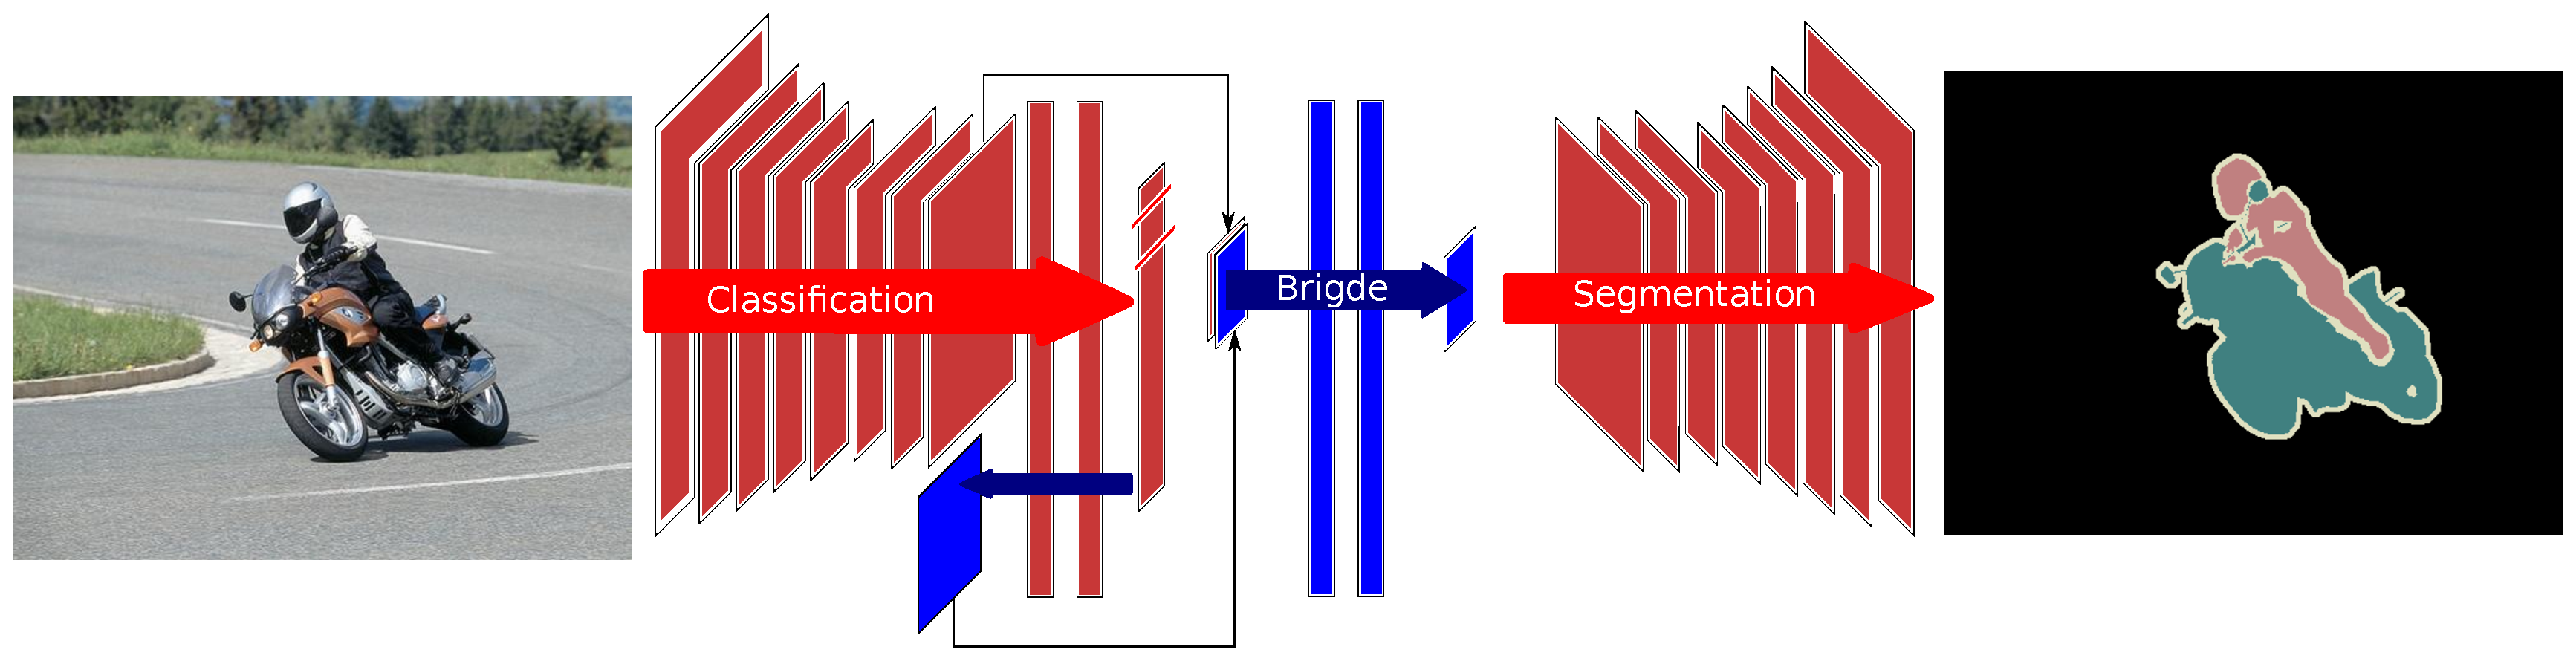
\includegraphics[scale=0.25]{hong}
 \caption{Architecture of the networks proposed in \textcite{hong2015decoupled}. Classification takes places through several convolution layers. Semantic segmentation uses deconvolutional layers to rebuild the original image.}
 \label{fig:hong}
\end{figure}
% show network architecture.

\textcite{hariharan2014hypercolumns} introduce the \textit{"Hypercolumn"} taken from neuroscience to also produce state of the art results. In order to overcome a problem with information from the last layers being too coarse, information from early layers must be also considered.  The hypercolumn allows to have information from several layers inside the CNN. It benefits from the trade-off between different layers by combining them. The last layers capture semantics in a more efficient way (category-level information), while the early layers help to obtain a more precise location (e.g. pose, illumination, articulation, location, etc.). The \textit{Hypercolumns} work as pixel descriptors, and were successfully used for diverse visual tasks (e.g. detection, segmentation, keypoint localization and part labeling).
Needless to say, it also uses multiple levels of abstraction and scale are necessary. This can be comparable to \textcite{farabet2013pami} mutli-scale pyramid.However the invariance in is similar, since the features come from the same level of the CNN. Figure ~\ref{fig:hyper} shows the hypercolumn idea implemented in a CNN. 

\begin{figure}
 \centering
 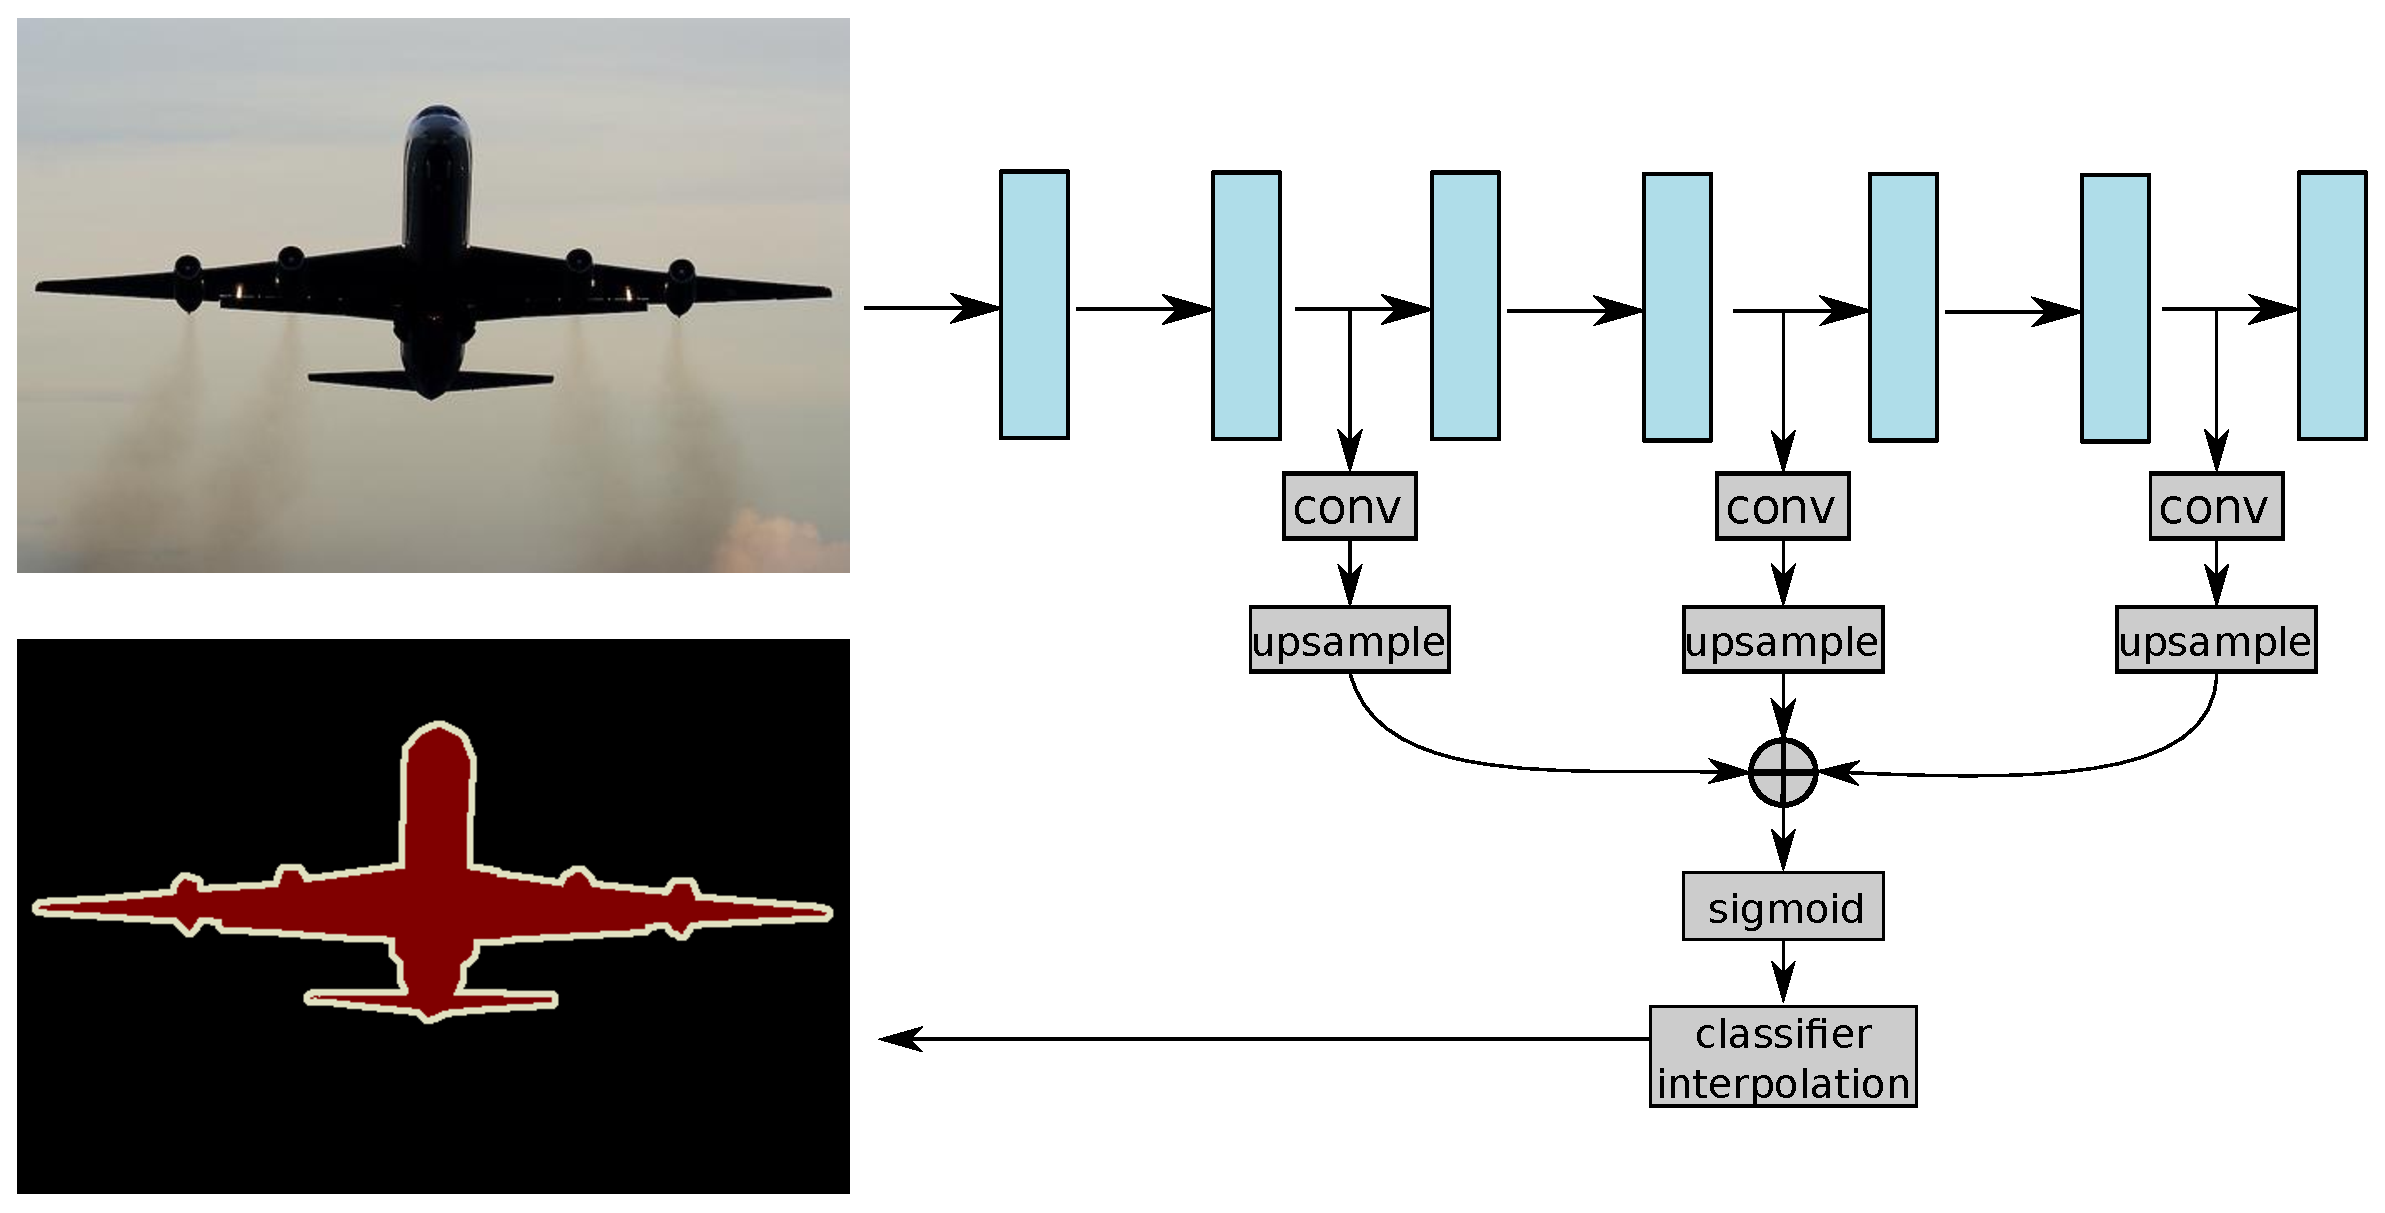
\includegraphics[scale=0.3]{hypercolumns}
 \caption{Original classification CNN is shown in blue, and added layers for the hypercolumn classifier are in gray (\textcite{hariharan2014hypercolumns}).}
 \label{fig:hyper} 
\end{figure}


Notably, \textcite{long2014fully} present an end-to-end system for semantic segmentation using only \textit{fully convolutional} networks. The models presented here are characterized for an architecture which combines deep, coarse, semantic informantion and shallow, fine, appearance information in a multi-layer framework. The fully convolutional models are obtained from  pre-trained CNN that perform image classification (\textcite{Krizhevsky_imagenetclassification}, \textcite{szegedy2014going} and \textcite{simonyan2014very}). In order to make them suitable for pixelwise classification, the inner product layers are replaced by convolutional layers, while a transfer of parameters occurs based on \textcite{donahue2013decaf}. A fine-tuning process is driven to adapt the fully convolutional networks for new semantic segmentation tasks. In order to produce finer segmentations, different layers are upsamled and fused. The main advantages of this approaches lay in the capacity of reusing learned values, reducing the need of a big training dataset (which is costly effort) and the use of Caffe. Figure ~\ref{fig:fcn} explains how semantic segmentation is possible with a fully convolutional net.

The approach of this thesis is based on \textcite{long2014fully}. Fully convolutional networks are possible to train using Caffe (\textcite{jia2014caffe}) as framework. Caffe allows to use pre-trained models, which are \href{https://github.com/BVLC/caffe/wiki/Model-Zoo}{publicly available} and well documented. It is also handy to choose this framework due the big communities of \href{https://groups.google.com/forum/#!forum/caffe-users}{users} and \href{https://github.com/BVLC/caffe}{developers}.  In order to make fine-tuning using a small dataset (\textcite{BrostowFC:PRL2008}) feasible, this thesis also makes use of transfer of parameters exposed in \textcite{donahue2013decaf}.  

\begin{figure}
 \centering
 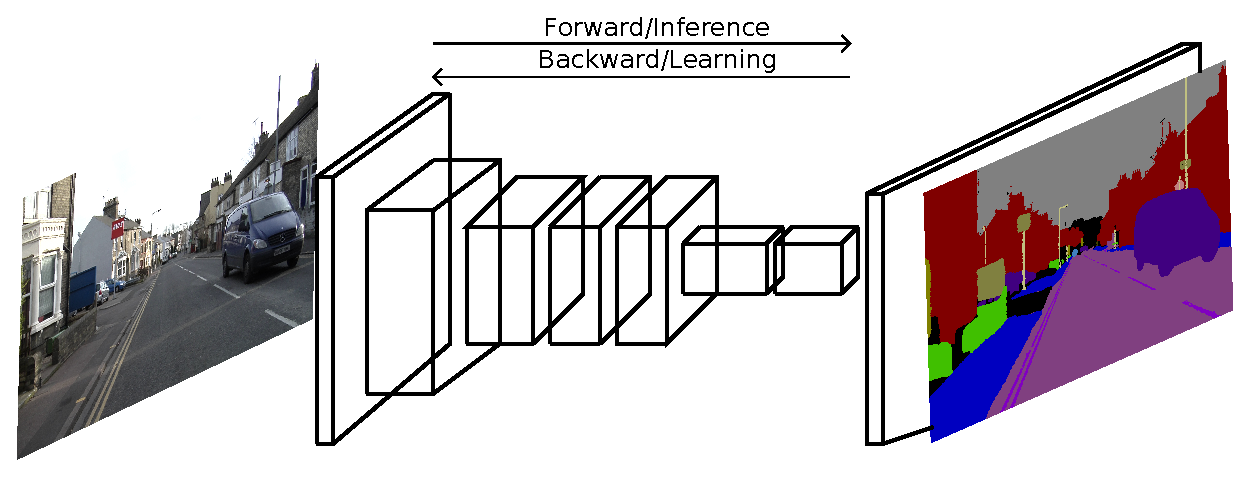
\includegraphics[scale=0.7]{camvid_convolution}
 \caption{Fully convolutional networks make dense predictions for pixel classification.The final layer makes use of a bilinear interpolation to produce the semantic segmentation}
 \label{fig:fcn}
\end{figure}
   

\section{Temporary Semantic Segmentation}
\label{sec:tempsemseg}
This section presents the approaches with state of the art results for temporary semantic segmentation. Since it is desired to yield a causal segmentation for online applications, omniscient methods are not covered due their inherent need of future frames. The purpose of this implementation is to enhance the traffic scene labeling using a temporary relation (besides the spatial relation from the CNN). The final result is expected to have avoid flickering segmentations and to increase the accuracy based on previous knowledge. Figure ~\ref{fig:causal} shows the desired kind of approach. %Add image with omniscient, causal and frame by frame.

%The taken approach is to adapt the CNN model for temporal fusion of the predicted outputs. The main idea behind such an approach is to overcome the traffic scene labeling not only by spatial relation but also using temporary relation in order to improve its performance.
 
\textcite{ess2009segmentation} is a work whose purposes are very similar to the ones from this thesis. A two-stages approach is introduced where the first stage generates a superpixel segmentation based on \textcite{felzenszwalb2004efficient}, which is later used in a second stage to construct a feature set for a classifier. The proposed image-based system is able to perform road recognition as well as a set of objects (e.g. cars, pedestrians, etc.). In order to allow online applications, the temporal smoothing is obtained using the forward pass output of a \textit{Hidden Markov Model} (HMM) \textcite{rabiner1989tutorial}.

\begin{figure}
 \centering
 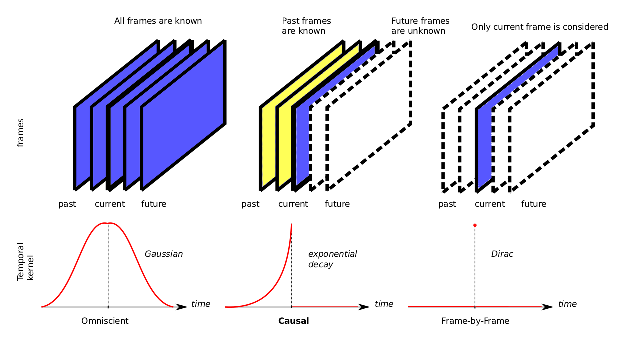
\includegraphics[scale=1.2]{segmentation_types}
 \caption{There are three types of video segmentation. In order to improve the segmentation performance, this thesis focuses on causal segmentation.}
  \label{fig:causal}
\end{figure} 

\textcite{paris2008edge} profit from the spatial-temporal dimensions mix from video datasets. This approach relies on a bilateral filtering and a mean-shift segmentation from \textcite{paris2007topological}. This is an online approach, therefore it only uses current and past data. The previously acquired data helps to ensure temporal coherence which otherwise cannot be accomplished by using frame-by-frame approaches.

\textcite{grundmann2010efficient} use a hierarchical graph-based algorithm in order to yield a temporary consistent segmentation. This algorithm addresses three problems: Temporal coherence, automatic tracking and scalability. Like similar approaches,  it is initialized with an oversegmentation using the graph-based image segmentation from \textcite{felzenszwalb2004efficient}. Afterwards, the algorithm makes use of Optical Flow (\textcite{horn1981determining}) to modify the graph structure with respect to time. A hierarchical segmentation yields a region grpah from a previous segmentation level.  This approach exhibits long-term temporal coherence and overcomes memory and runtime 

%\textcite{karpathy2014large} have successfully used CNNs to classify videos. This work denoted how it is possible to take advantage of local-tempral information within the CNNs.
\textcite{miksik2013efficient} perform a scene analysis generating predictions of semantic categories over time. These predictions are characterized for being spatially and temporally consistent. It is an online algorithm which uses a temporal filter based on exponential smoothing over past predictions. This method can be applied in combination with any frame-by-frame analysis technique, as long as it produces a pixelwise labeling. This temporally smoothing technique works using Optical Flow (\textcite{horn1981determining}) to estimate correspondances with the previous frame.
  
\textcite{couprie2014convolutional} propose an approach whose objectives are similar to the ones of this thesis. It yields real-time segmentation of indoor scenes. This method benefits from the semantic segmentation of \textcite{farabet2013pami}. In order to improve the performance of the segmentation, the temporal consistency of the video sequences is exploited. This causal segmentation is taken from \textcite{couprie2013causal} and uses the superpixel segmentation method from \textcite{felzenszwalb2004efficient}. A graph-matching technique is developed in order to match previous segmentations and to enrich the current frame segmentation. The main advantages of this approach are the computational efficiency and the possibility of future implementations working together with another frame-by-frame technique.

The method developed in this thesis, makes use of the causal segmentation proposed in \textcite{couprie2013causal}, due its capabilities for real-time implementations and the availability of the \href{http://perso.esiee.fr/~coupriec/code.html}{programming code}. 



%
%
%



% #######################################################
% !TeX encoding = ISO-8859-1
%%%%%%%%%%%%%%%%%%%%%%%%%%%%%%%%%%%%%%%%%%%%%%%%%%%%%%%%%%%%
\chapter{Theoretical Framework}
\label{ch:thefram}
This chapter presents a theoretical definition of all the main concepts used in the implementation of a traffic scene understanding system.

The section ~\ref{sec:cnn} covers the theoretical principles of Convolutional Neural Network and how they yield a semantic labeling process. Applications not related to computer vision tasks are beyond the scope of this thesis and omitted.

Section ~\ref{sec:secseg} explains several segmentation methods used in the temporary consistent segmentation. Efficient graph-based segmentation from \textcite{felzenszwalb2004efficient} and Watershed cuts as described in \textcite{cousty2009watershed}. These segmentation methods are characterized for requiring a small computationally effort and being fast enough to allow their use in real-time applications.  

To end this chapter, section ~\ref{sec:tempconsseg} describes how causal segmentation is yield (e.g. previous frames matching, Optical Flow and combined used with frame-by-frame approach). 
%In order to clarify how the traffic scene understanding is done via semantic segmentantion, Convolutional Neural Networks (CNNs), Efficient Graph-based segmentation, Optical flow and Causal Segmentation are explained in detail in the subsequent sections. 
%In this Chapter the basics of Convolutional Neural Networks are first presented for a better understanding of the chosen semantic segmentation approach. Explanation of how Neural Networks were modified in order to handle vision tasks. The uses of Convolutional Neural Networks will often focus on this work needs. Some other applications for Convolutional Neural Networks are beyond the scope of this thesis. \textcite{szegedy2014going} 

\section{Convolutional Neural Networks}
\label{sec:cnn}

Convolutional Neural Networks (CNNs) are Neural Networks which perform a \textbf{convolution instead of a matrix multiplication in at least one of their layers} (\textcite{Bengio-et-al-2015-Book}). In order to process data inside a CNN, this must have a grid-like topology. CNNs are loosely based on neuroscientific principles and inspired on the mammalian vision system.

CNNs were firstly introduced in \textcite{fukushima1980neocognitron}, but it was until \textcite{le1990handwritten} (introduction of backpropagation) and \textcite{lecun1998gradient} where they were successfully implemented to solve visual tasks.
After the first CNN implementation with GPU in  \textcite{ciresan2011flexible}, this deep learning method started to achieve a state of the art performance and consequently better results than traditional approaches. 

The many arguments in CNNs are: the inputs, kernels and the outputs, which are also known as \textit{Feature Map}. The inputs are multidimensional array of data, while the kernels are a multidimensional array of parameter that can be learned.

Due the inherent nature of a CNN model, the memory requirements diminish, the statistical efficiency is improved and fewer parameters are used compared to traditional Neural Network models. This is due the sparse interactions product of a kernel several times smaller than the input. The mathematical concept is defined in subsection ~\ref{subsec:convop}

\subsection{Convolution Operation}
\label{subsec:convop}
The convolution operation used in CNNs differs from the definition used in some other fields (e.g. Engineering, Mathematics). \textit{Convolution} is an operation on two functions of a real-valued argument. It is represented in equation ~\ref{equ:convo}:
%
\begin{equation}
 s(t) = \int x(a)w(t-a)da
 \label{equ:convo}
\end{equation}

However the convolution operations is often denoted with an asterisk, like in equation ~\ref{equ:convi}:

\begin{equation}
 s(t) = (x \ast w)(t)
 \label{equ:convi}
\end{equation}
 
In convolutional network terminology, the argument \textit{x} is known as the \textit{input} and the other argument \textit{w} as the \textit{kernel}. The output \textit{s(t)} is referred as \textit{feature map}.
In machine learning applications , the input and the kernel are multidimensional arrays.
Since convolution is used for two-dimensional images:

\begin{equation}
 s[i,j] = (I \ast K)[i,j] = \sum_{m} \sum_{n}I[m,n]K[i-m,j-n]
 \label{equ:convii}
\end{equation}

Another view is more straightforward for a machine learning library implementation. Due the commutative property of the convolution operation, (\ref{equ:convii}) is equivalent to:

\begin{equation}
 s[i,j] = (I \ast K)[i,j] = \sum_{m} \sum_{n}I[i-m,j-n]K[m,n]
 \label{equ:convoo}
\end{equation}

Where \textit{I} is the two-dimensional image and \textit{K} is the two-dimensional Kernel.
The commutative property is not fundamental for a neural network implementation. Neural network libraries have an operation called \textit{cross-correlation}, which is the same as a convolution with no kernel flip as can be seen in equation ~\ref{equ:crosscor}. Many machine learning applications implement cross-correlation, but address it as convolution.

\begin{equation}
 s[i,j] = (I \ast K)[i,j] = \sum_{m} \sum_{n}I[i+m,j+n]K[m,n]
 \label{equ:crosscor}
\end{equation}

\begin{figure}
 \centering
 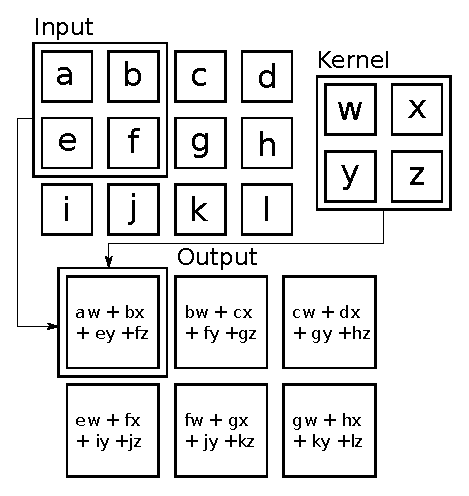
\includegraphics[scale=1]{crosscorrelation}
 \caption{2-D convolution.}
 \label{fig:crosscor}
\end{figure}

Figure ~\ref{fig:crosscor} show how a 2-D convolution takes place with no kernel-flipping. It can also be noticed that due the smaller kernel size, the convolution operation correspond to a sparse matrix. Most Neural Network models allow to easily replace a matrix multiplication with a convolution (as long as the model does not depend on specific matrix structures).
Convolution can be seen as a multiplication by a matrix, nevertheless the matrix has its entries constrained . For unidimensional convolution this is known as \textit{Toeplitz matrix}.For a 2-D convolution operation the \textit{doubly block circular matrix} is the analogue.  
Convolution can be seen as multiplication by a matrix with several constrained entries (e.g. Univariate discrete convolution is constrained to be a \textit{Toeplitz matrix}).
A convolution in two dimensions corresponds to a \textit{doubly block circular matrix}. 

Typical CNN models make use of more specialized stages in order to deal with large data inputs. These stages perform different operations and together form a \textit{Convolutional layer}. Convolutional layers are explained in the following subsection ~\ref{sub:convmod}.

\subsubsection{Variants of the Convolution function}
As explained in the past section ~\ref{subsec:convop}, the functions used in CNNs differ slightly from the convolution operation in the mathematical literature. 
First of all, there are several convolution operations which run in parallel, this is due the kernel properties. A kernel can only extract one kind of features, therefore multiple convolutions in a layer help to obtain many kind of features.
Also the inputs are generally a grid of vector-based observations rather than real values. When working with images, the inputs and outputs are represented as 3-D tensors, with one index for the different channels (i.e. red, green and blue) and the other two indices for the spatial coordinates.
In equation ~\ref{equ:varconv}, ${K_{i,j,k,l}}$ is the kernel, which gives the connection strength between a unit in channel \textit{i} of the output and a channel \textit{j} of the input, with an offset of \textit{k} rows and \textit{l} between the output and the unit. The input data is formed by the elements ${V_{i,j,k}}$, where \textit{i} indicates the channel and \textit{j} and \textit{k} indicate  rows and columns respectively. The convolution is assumed without kernel flipping. 

\begin{equation}
 {Z_{i,j,k}} = \sum_{l,m,n}{V_{l,j+m,k+n}}{K_{i,l,m,n}}
 \label{equ:varconv}
\end{equation}

In order to reduce computational costs, it is possible to skip over some positions of the kernel (the feature extraction becomes coarse). It can be seen as a downsampling in the convolution and appears in equation ~\ref{equ:downconv}. The \textit{s} is referred as the stride and allows to sample only every \textit{s} pixels in each direction of the output.

\begin{equation}
 {Z_{i,j,k}} = \sum_{l,m,n}[{V_{i,j \times s+m,k \times s+n}}{K_{i,l,m,n}}]
 \label{equ:downconv}
\end{equation}

Zero-pad is one essential feature of the convolution that should be implement at the input in order to make it wider. The width of the representation is reduced by the kernel width - 1 at each layer if zero padding is not implemented. Therefore zero padding avoids the necessity to choose between shrinking the spatial representation and using small kernels. 

In order to perform learning in a convolutional neural network, other operations are required. A Computation of gradients with respect to the kernel, given the gradients with respect to the output must be yield. 

\begin{figure}
 \centering
 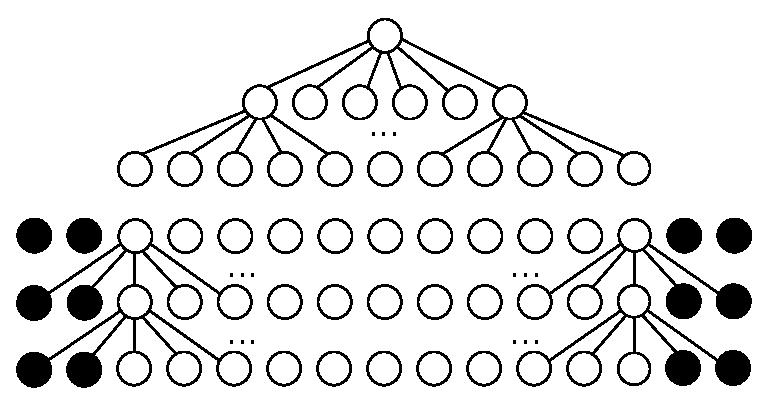
\includegraphics[scale=1]{zero-padding}
 \caption{\textit{Zero Padding effect:} \textbf{TOP:} Zero padding is not implemented,, therefore the network shrinks its size. \textbf{BOTTOM:} Zero padding prevents the network from shrinking with depth.}
 \label{fig:zp}
\end{figure}

\subsection{Convolutional Layer}
\label{sub:convmod}
CNN models are composed of several layers, where at least one of them is a \textit{convolutional layer}. Convolutional layers have these stages:
\begin{itemize}
 \item Convolution stage
 \item Detector stage
 \item Pooling stage
 \item (Local Response Normalization stage)
\end{itemize}

The norm stage appears in brackets because it is not always present in a convolution layer. However, it is present in several architectures. Figure ~\ref{fig:convlay} shows how all the stages inside a convolutional layer are interconnected. The convolution stage is already explained in ~\ref{subsec:convop} and the rest of the stages are explained below.
  
\begin{figure}
 \centering
 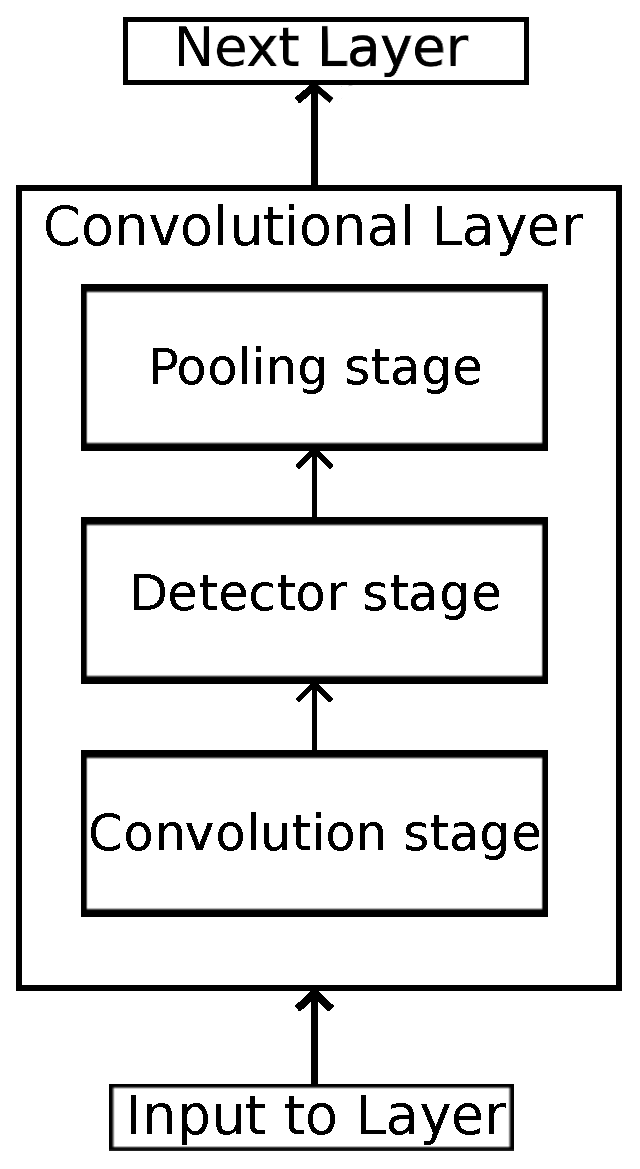
\includegraphics[scale=0.3]{convolutional_layer}
 \caption{Each convolution layer is divided into three stages.}
 \label{fig:convlay}
\end{figure}

\subsubsection{Detector stage}
\label{subsub:detector}
In the detector stage an \textit{activation function} is performed. An activation function defines an output for a given input or set of inputs. There are three main kinds of activation functions:
\begin{itemize}
 \item \textit{Hyperbolic tangent function (Tanh)}:
  \begin{equation}
   f(x) = \frac{e^{x}-e^{-x}}{e^{x}+e^{-x}}
   \label{equ:tanh}
  \end{equation}
 \item \textit{Logistic sigmoid function}:
   \begin{equation}
    f(x) = \frac{1}{ 1 + e^{-x}}
    \label{equ:sigmoid}
   \end{equation}   
 \item \textit{Rectified Linear Unit function (ReLU)}:
  \begin{equation}
   f(x) = max(0,x)
   \label{equ:relu}
  \end{equation}
 \item \textit{Parametric Rectifier Linear Unit function (PReLU)}:
  \begin{equation}
  f(x) =\begin{cases} ax & \mbox{if } x \leq 0 \\ x & \mbox{if } x > 0 \end{cases}     
  \label{equ:prelu}
  \end{equation}     
\end{itemize} 

In equations ~\ref{equ:tanh}, ~\ref{equ:sigmoid}, ~\ref{equ:relu} and ~\ref{equ:prelu}; \textit{x} represents the input and \textit{f(x)} is the respective output. The behavior of each activation function can be observed in Figure ~\ref{fig:actfct}. All of these functions are widely used for deep learning, but only the last two (ReLU and PReLU) are nowadays used for Convolutional Neural Networks. Therefore \textit{tanh} and \textit{sigmoid} functions are not covered. In order to coincide with \textcite{Bengio-et-al-2015-Book} the rectifier functions will be referred as  \textit{Detector stage}.

\begin{figure}
 \centering
 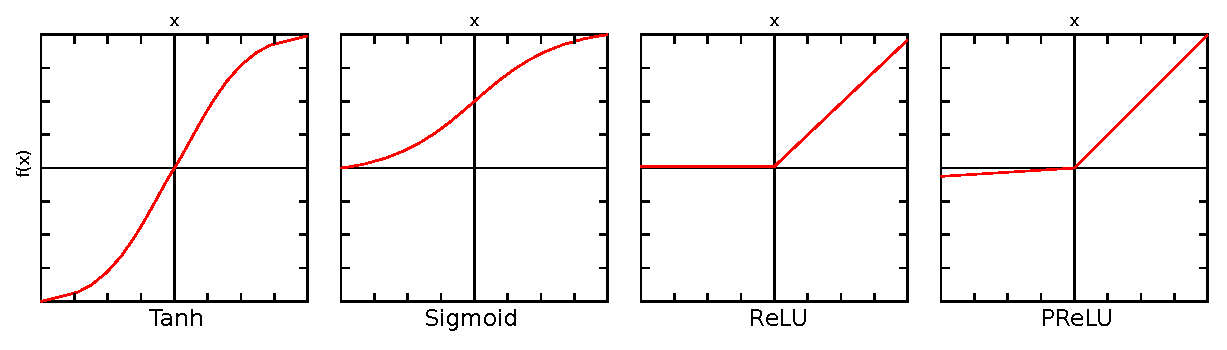
\includegraphics[scale=0.7]{activation_fct}
 \caption{The different types of activation functions used in Convnets.}
 \label{fig:actfct}
\end{figure}

% There is no clear understanding of how and why a CNN works, usually better perfomance is achieved by trial-and-error 
\textcite{zeiler2013rectified} mention and prove empirically how CNNs benefit from ReLU functions. The nature of ReLU functions allows to easily train deep networks (even from random initialization). Equation ~\ref{equ:relu} transform the system into a linear system since it only focuses on non-zero units. ReLU also yield a more regularized internal representation (zero-outputs are often produced, if there is misalignment between inputs and internal weights).   state that there are two reasons for ReLU to be beneficial for efficient learning of deep neural networks. The first reason is the system reduction to a linear convex system (it only focuses on units that are non-zero). The other reason is a more regularized internal representation. ReLU often produce zero-outputs, if the input is not aligned with the internal weights.

According to \textcite{glorot2011deep} ReLU units are suitable for CNNs due the sparsity of data, an inherent property of the convolution operation. It is worth to mention that not only vision tasks obtain a performance improvement, but also acoustic models (\textcite{maas2013rectifier}) and speech processing (\textcite{zeiler2013rectified}). It becomes obvious that Rectified Linear units are a must in order to yield state of the art results while using CNNs. 
%PReLU is trained and optimized using backpropagation (\textcite{le1990handwritten}) just as the other layers 
%\begin{equation}
% \frac{\partial \varepsilon}{\partial {a_i}} = \sum\limits_{y_i} \frac{\partial \varepsilon}%{\partial f({x_i})} \frac{\partial f({x_i})}{\partial {a_i}}
%\end{equation}

The Parametric Rectified Linear Unit (PReLU) is shown in figure ~\ref{fig:actfct} and can be seen as modified version of the ReLU function. It succesfully surpassed the performance achieved by  ReLU based CNN models (\textcite{he2015delving}). Its implementation improves model fitting with almost no extra computational effor and reducing the overfitting risk. PReLU Robustness lies in the \textit{a} parameter from equation ~\ref{equ:prelu} which is learnable. This is similar to the Leaky Rectified Linear Unit (LReLU) proposed in \textcite{maas2013}, which uses a small fixed value (\textit{a =  0.01}) to avoid zero gradients; but when comparing to ReLU only PReLU performance has a significant impact. In PReLU, only by adding few parameters with a negligible computation cost, a CNN performance is improved due the adaptative learning of activation function shapes.  
%According to \textcite{glorot2011deep}, ReLU are suitable for CNNs since they benefit from sparse data, an inherent property of the convolution operation. They proved their efficiency not only in vision tasks, but also in acoustic models (cite Maas), \textit{Restricted Bolzmann Machines (RBM)} (cite V. Nair) and also speech processing (cite Zeiler). Therefore this detector stage becomes essential for state of the art neural networks. 
%Neural Networks are special case of program paradigms. Their singularity lies inside the learning capability from observed data. Despite being invented several years ago, it was recently when they started to achieve a better perfomance than some other traditional approaches. These new techniques are the now so called deep neural networks.

%Deep Learning and Deep Neural Networks are nowadays in development and still reaching outstanding performance on many problems (i.e. Computer Vision, Speech Recognition, et cetera.)

%Convolutional Neural Networks (CNNs) process data with a grid-like topology. The name implies that a mathematical operation called "convolution" is yield. CNNs use convolution instead of general matrix multiplication. (Cite Bengio)

%For CNNS, the first argument in a convolution is called input and the second argument is referred as kernel. The output is known as Feature Map.

%Inputs are usually multidimensional arrays of data and Kernels are mutlidimensional array of parameters that can be learned.

%CNNS have sparse interactions "sparse connectivity/weights" due a kernel smaller than the input. This allows to save fewer parameters, reduces memory requirements and improves statistical efficiency 

%insert ReLU eps and tanh, sigmoid function plots

\subsubsection{Pooling stage}
\label{subsub:pool}
As shown in figure ~\ref{fig:convlay}, the convolution layer is formed of convolution, detector and pooling stage. The pooling stage modifies the output of the layer further. It replaces the output in a certain location with a statistical summary of the nearby outputs. 
The Pooling stage comes after the Detector stage. It replaces the output in a certain location with a statisctial summary of the nearby outputs. Its purpose is to reduce the invariance caused by small translations inside the inputs. The most common pooling functions are:

\begin{itemize}
 \item \textit{Max function}: Maximum output within a rectangular neighborhood.
 \item \textit{L2 norm function}: Squared root of the absolute values squared.
 \item \textit{Average function}: Average output of a rectangular neighborhood.
 \item \textit{Weighted average function}: Output based on the distance from the central pixel.
\end{itemize}

Invariance to local translation has been proved to be an important property if the vision task focuses more on the presence of a feature rather than in its location. However depending on the task to preserve the location of a feature is desired.
Pooling summarizes over an output neighborhood allow to use fewer pooling stages than detector stages . Figure ~\ref{fig:maxpool} shows how this summarization generates an increased computer efficiency and reduced memory requirements because the next layer will have fewer parameters to process. The figure depicts a max-pooling operation with a pool width of three and a stride between pools of two. 

Convolution and Pooling can cause underfitting, therefore state of the art models (e.g \textcite{Krizhevsky_imagenetclassification} and \textcite{szegedy2014going}) are designed to use pooling on some channels. This yields highly invariant features and features which are non prone to underfitting

\begin{figure}
 \centering
 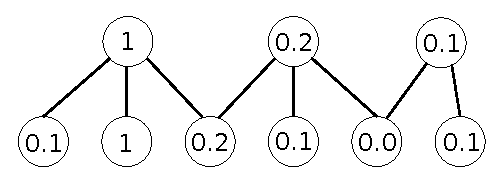
\includegraphics[scale=1]{maxpooling}
 \caption{Pooling with downsampling}
 \label{fig:maxpool}
\end{figure}

\subsubsection{Local Response Normalization (LRN)}
\label{subsub:LRN}
Response normalization is implemented as a form of lateral inhibition, and is inspired on the real neurons. \textcite{hinton2012improving} introduced this type of layer in order to encourage competition for large activations amongst neuron outputs which are computed using different kernels. In order to yield a better generalization, the local normalization is performed as in equation ~\ref{equ:LRN}.$b^i_{x,y}$ represents the  response-normalized activity, $a^i_{x,y}$ denotes the activity of a computed neuron, where $i$ is the kernel and $(x,y)$ the position coordinates. The sum runs over $n$ kernel maps at the same spatial position and $N$ stands for the number of kernels in the layer.  

\begin{equation}
 b^i_{x,y} =  a^i_{x,y}/ \bigg( k+\alpha\sum\limits_{j=max(0,i-n/2)}^{min(N-1,i+n/2)}(a^j_{x,y})^2 \bigg) ^\beta
 \label{equ:LRN}
\end{equation}

The constanst $k$,$n$,$\alpha$ and $\beta$ are hyperparameters which are calculated using a validation set. A LRN layer follows a ReLU layer, though ReLU units do not require input normalization, but as \textcite{Krizhevsky_imagenetclassification} implemented it prevents saturating inputs.
  
\subsection{Deconvolutional Layer}
\textcite{zeiler2011adaptive} proposes this novel architecture which uses the same components of a convolutional layer (See section ~\ref{sub:convmod}) but in reverse. Originally used to perform unsupervised learning, the deconvolutional layers are later used as a visualization technique in CNNs. This approach appears in \textcite{zeiler2014visualizing}. It allows to to find the performance contribution of a layer, and have also been used in image segmentation tasks (e.g. \textcite{long2014fully}, \textcite{noh2015learning}) 

Equation ~\ref{equ:deconv} shows how the reconstruction $\hat{y_1}^c$, where $c$ represents the color channels, is performed by the sum of  convolution operations of the feature maps $z_{k,1}$ with filters $f^c_{k,1}$. 
\begin{equation}
 \hat{y_1}^c = \sum\limits_{k=1}^{K_1}z_{k,1}\ast f^c_{k,1}
 \label{equ:deconv}
\end{equation}

The deconvolution tries to minimize the reconstruction error under a sparsity constraint and a set of feature maps. This is explained in equation ~\ref{equ:deconvcost}. $C_l(y)$ stands for the cost function and comprises two terms weighted by $\lambda_l$ a likelihood which keeps the $\hat{y}_t$ reconstruction close to $y$ input, and a regularization term of the feature maps $z_{k,l}$. 
 
\begin{equation}
 C_l(y) = \frac{\lambda_l}{2} ||\hat{y}_l-y||^2_2+\sum\limits_{k=1}^{K_t}|z_{ĸ,l}|_1
 \label{equ:deconvcost}
\end{equation}

Figure ~\ref{fig:deconv} explains how a deconvolutional layer works. The activities performed in a convolutional layer are mapped back to the pixel space. The stages are performed successively in this order: unpooling, rectifying and filter.

\begin{figure}
 \centering
 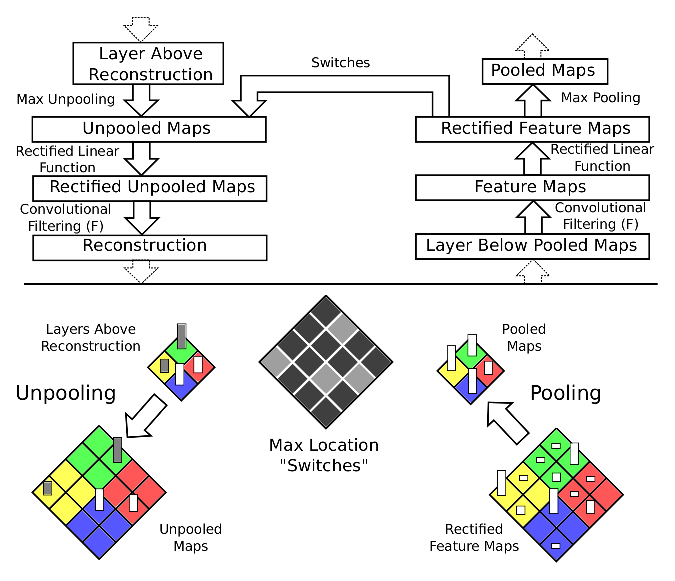
\includegraphics[scale=1]{deconvolution}
 \caption{\textbf{LEFT}: deconvolutional layer. \textbf{RIGHT}: convolutional layer. The deconvolution layer yields an approximate reconstruction of the layer beneath convolution layer.
 \textbf{BOTTOM}: This diagram depicts the unpooling operation in the deconvolutional layer. The black/gray squares are negative/positive activations in the feature map (\textcite{zeiler2014visualizing}).}
 \label{fig:deconv}
\end{figure}

\section{Convolution parameters}
\subsubsection{Dropout}
Another addition to the convolutional neural networks is the so called \textit{dropout layer}. Deep neural nets are characterized for having a large number of parameters, therefore the nets are prone to overfitting. In order to address the overfitting problem, there are several techniques that can be implemented (e.g. soft weight sharing, penalties like L1 and L2 regularization, stop the training if the performance in the validation data is reduced).

It is possible to "regularize" a model by averaging the predictions of all possible setting of the parameters. This works well for small models, however the use of this technique on a several number of learned models that share parameters (i.e. Model combination) is computationally expensive.
 
\textcite{srivastava2014dropout} proposed the \textit{Dropout} technique in order to address the two cited problems (i.e. overfitting and high computational effort). It also allows to combine many different neural networks architectures in an efficient way. Figure ~\ref{fig:dropout} depicts the dropout technique, which can be define as the drop out  of units in a neural network.  Normally each unit is retained with a fixed probability \textit{p} (usually set at 0.5) in order to be optimal for many kinds of networks and tasks. A Neural Network trained with the dropout technique can be seen as a collection of $2^n$ thinned networks, each of which shares its weights. 

\begin{figure}
 \centering
 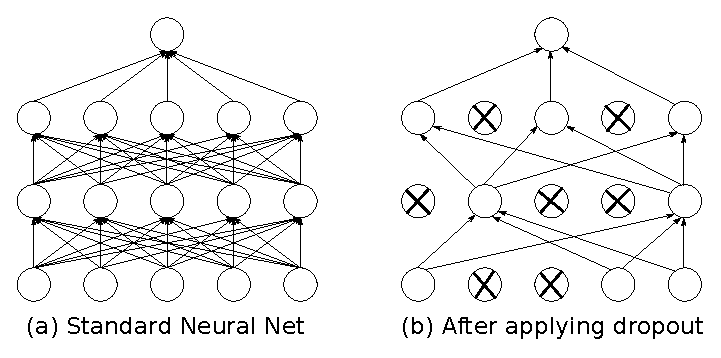
\includegraphics[scale=1]{dropout}
 \caption{\textbf{Left}: A standard neural net with 2 hidden layers. \textbf{Right}: An example of a thinned net, producht of the dropout technique.}
 \label{fig:dropout}
\end{figure}

A model where dropout is performed can be described as follows: Given \textit{L} hidden layers, let $l\in\{1,...,L\}$ index the hidden layers. $z^l$ and $y^l$ are vectors of inputs into layer $l$ and outputs from layer $l$ respectively. $w^l$ and $b^l$ represent the weights and biases at layer $l$. Feed forward operation of a standard neural network is then described in equations ~\ref{equ:do1} and ~\ref{equ:do2}.
  
\begin{equation}
 {z_i}^{(l+1)} = {w_i}^{(l+1)}y^l+{b_i}^{(l+i)}
 \label{equ:do1}
\end{equation}

\begin{equation}
 {y_i}^{(l+1)} = f({z_i}^{(l+1)})
 \label{equ:do2}
\end{equation}

where $f$ is an activation function, like the ones seen in the detector section ~\ref{subsub:detector}. The feed-forward operation in a network where dropout looks like this:  

\begin{equation}
 {r^l_j} \sim Bernoulli(p)
 \label{equ:do3}
\end{equation}

\begin{equation}
 \tilde{y}^l = r^l \ast y^l
 \label{equ:do4}
\end{equation}

\begin{equation}
 {z_i}^{(l+1)} = {w_i}^{(l+1)}\tilde{y}^l+{b_i}^{(l+1)}
 \label{equ:do5}
\end{equation}

\begin{equation}
 {y_i}^{(l+1)} = f({z_i}^{(l+1)})
 \label{equ:do6}
\end{equation}

Equation ~\ref{equ:do3} shows a $r^l$, which is a vector of random variables that have a probability $p$ of being 1. In equation ~\ref{equ:do4}, $\ast$ denotes an element-wise product. The vector $r^l$ is sampled and multiplied with the outputs $y^l$ of that layer, to create a thinned output $\tilde{y}^l$. This process is applied at each layer and the outputs are used as inputs for the next layer.

The training of the dropout units is similar to the Stochastic Gradient Descent method used in standard neural networks. Forward and backpropagation are done on the thinned networks, while the gradients for each parameter are averaged over the training cases. Momentum, annealing learning rates and L2 weight decay are also useful to omprove the stochastic gradient descent. The noise generated by the dropout allows the optimization to be most robust by exploring different regions of the weight space. 

It must be noticed that dropout introduces noise in the gradients if compared to the standard stochastic gradient descent (i.e. some grandients cancel each other). In order to overcome this issue, the learning rate should be increased 10-100 times and a high momentum must be chosen. This increase the speed of the learning process.

Nevertheless, the dropout technique in neural network has its drawbacks. The training process is 2-3 longer due a very noisy parameter update. Each training case focuses on a specific random architecture, therefore the calculated gradients are not the same gradients used in the final architecture. There is a trade-off between training time and overfitting that should be analyzed depending the characteristics of a given neural network (i.e. dataset, architecture).    

\subsection{Learning}
The forward pass and backward propagation are the main operations being yield in a neural network.

The forward pass computes the output given the input for inference.
\begin{equation}
 fw(x) = h(g(x))
 \label{equ:FWD}
\end{equation}

The backward pass \textit{(back-propagation)} computes the gradients given the loss for learning

\begin{equation}
 \frac{\partial{fw}}{\partial{h}} \frac{\partial{fw}}{\partial{W_{ip}}} \frac{\partial{fw}}{\partial{g}}
\end{equation}

\begin{figure}
 \centering
 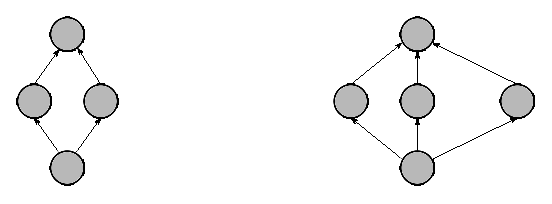
\includegraphics[scale=1]{backprop}
 \caption{backpropagation}
\end{figure}
\subsubsection{Loss functions}
\label{sec:loss}
A loss function evaluates the quality of the learning by mapping parameter settings to a scalar value, to test the \textit{accuracy} of the learned parameters. The goal of the learning process is to find a set of parameters which minimizes the loss function.

When Neural Network models started to become popular, the most used loss function was the Least Squared Error (LSE) $L(f_w(x),y) = ||f_w(x)-y||^2$. Nevertheless this is not effective if the values of $y$ are discrete (i.e. classification tasks), and therefore other loss functions should be employed.

\subsubsection{Softmax}
\label{sec:softmax}
\begin{equation}
 p = softmax(a) \Longleftrightarrow p_i = \frac{e^{a_i}}{\sum_j e^{a_j}}
 \label{equ:softmax}
\end{equation}

Equation ~\ref{equ:softmax} is the \textit{softmax} (\textcite{bridle1990probabilistic}) and its purpose is to specify multiple Bernoulli (\textit{multinoulli}) distributions. Where $a$ is a set of activations 

The softmax loss layer is conceptually identical to the softmax layer applied before a multinomial logistic layer. It is the loss function used in Caffe



\subsection{Optimization}
The backward pass defines how to compute the gradient of the loss with respect to the model parameters. However, in order to update the weights of a Neural Network, gradient-based learning algorithms need to be implemented. 
Though several learning algorithms for deep neural networks exist, this thesis only covers some of them due their popularity and therefore further implementation in Caffe
\subsubsection{Stochastic Gradient Descent (SGD)}
\label{subsub:SGD}
Stochastic Gradient Descent is a widely used optimization algorithm for machine learning. It uses a stochastic estimator of the gradient in order to perform an update.  

\textit{empirical risk} $E_n(f)$ measures the training set performance, while the \textit{expected risk} $E(f)$ calculates the expected performance on future examples. Both appear in equation ~\ref{equ:risk}
\begin{equation}
 E(f)= \int l(f(x),y)dP(z) \hspace{2cm} E_n(f) = \frac{1}{n}\sum\limits_{i=1}^nl(f(x_i),y_i)
 \label{equ:risk}
\end{equation}
Gradient Descent (GD) minimizes the empirical risk $E_n(f_w)$. In each iteration the weights $w$ on $E_n(f_w)$ are updated as in equation ~\ref{equ:1GD}:
\begin{equation}
 w_{t+1} = w_t-\gamma\frac{1}{n}\sum\limits_{i=1}^n\nabla_wQ(z_i,w_t),
 \label{equ:1GD}
\end{equation}
$\gamma$ represents the learning rate, which achieves \textit{linear convergence} in case of being sufficiently small and in conjunction with a $w_o$ close to the optimum.
If the scalar learning rate $\gamma$ is replaced by a positive matrix $\Gamma_t$ a better optimization can be designed. Equation ~\ref{equ:2GD} shows a \textit{second order gradient descent}. 
\begin{equation}
 w_{t+1}= w_t-\Gamma_t\frac{1}{n}\sum\limits_{i=1}^{n}\nabla_wQ(z_i,w_t).
 \label{equ:2GD}
\end{equation}

Stochastic Gradient Descent is a widely used optimization algorithm for machine learning. It uses a stochastic estimator of the gradient in order to perform an update. It is also known as \textit{online gradient descent} . It is a drastic simplification since each iterations estimates the gradient based on single random $z_t$:
\begin{equation}
 w_{t+1} = w_t - \gamma_t \nabla_w Q(z_i,w_t)
 \label{equ:SGD}
\end{equation}
The SGD optimizes the expected risk, due the fact that the examples are randomly drawn from a ground truth distribution. The randomly drawn examples introduces noise, therefore the SGD gradient does not become 0 even when a minimum is reached.

The learning rate $\gamma_t$ is a crucial hyperparameter, which sometimes must be allowed to decrease its size in order to converge to a minimum. 

Since the data sizes grow faster than the processing speed, Stochastic Gradient Descent have become popular. This is due its performance, which is good enough if the training time is the bottleneck.

\begin{equation}
 w_{t+1}=w_t-\gamma_t\Gamma_t\nabla_wQ(z_t, w_t)
 \label{equ:2SGD}
\end{equation} 

\begin{center}
\begin{tabular}{| l |}
\hline
 \textbf{Stochastic Gradient Descent (SGD)}\\
\hline
 \textbf{Require:} Learning rate $\gamma_t$\\
 \textbf{Require:} Initial parameter $w_t$\\
 \hspace{1cm}\textbf{while} Stopping criterion not met \textbf{do}\\
 \hspace{2cm}Sample a minibatch of $t$ examples from the training set $\textbf{z}_{(1)} ,...,        \textbf{z}_{(t)}$ \\
 \hspace{2cm}Set \textbf{$f(t) = 0$}\\
 \hspace{2cm}\textbf{for} i = 1 to $t$ do\\
 \hspace{3cm}Compute gradient estimate: $f(t+1) = f(t) + \nabla_w Q(z_i,w_t)$\\
 \hspace{2cm}\textbf{end for}\\
 \hspace{2cm}Apply update: \textbf{$w_{t+1} = w_t - \gamma_t f(t+1)$}\\
 \hspace{1cm}\textbf{end while}\\
\hline
\end{tabular}
\end{center} 

\textbf{Table with SGD Algorithm}
\textcite{bottou2012stochastic} \textcite{Bengio-et-al-2015-Book} \textcite{Krizhevsky_imagenetclassification} 

\subsubsection{Momentum}
\label{subsub:moment}
Momentum helps to overcome inherent weaknesses of the stochastic gradient descent strategy. One of the main drawbacks of SGD is the slow training time, which is particularly slow when the gradient is small. 

Momentum function is to speed up the learning process 

\begin{center}
\begin{tabular}{| l |}
\hline
 \textbf{Stochastic Gradient Descent (SGD) with momentum}\\ 
\hline
 \textbf{Require:} Learning rate $\gamma_t$, momentum parameter $\alpha$\\
 \textbf{Require:} Initial parameter $w$, inivital velocity $v$\\
 \hspace{1cm} \textbf{while} Stopping criterion not met \textbf{do}\\
 \hspace{2cm} Sample a minibatch of $t$ examples from the training set  $\textbf{z}_{(1)} ,...,        \textbf{z}_{(t)}$ \\
 \hspace{2cm} Set $\textbf{f(t) = 0}$\\
 \hspace{2cm} \textbf{for} $i=1$ to $t$ \textbf{do}\\
 \hspace{3cm} Compute gradient estimate: $f(t+1) = f(t) + \nabla_w Q(z_i,w_t) $\\
 \hspace{2cm} \textbf{end for}\\ 
 \hspace{2cm} Compute velocity update: \textbf{$v = \alpha v-\gamma_t f(t+1)$}\\
 \hspace{2cm} Apply update: \textbf{$w_{t+1} = w_t + v$}\\
 \hspace{1cm} \textbf{end while}\\
\hline
\end{tabular}
\end{center}



\subsubsection{Adaptative Gradient (AdaGrad)}
\label{subsub:AdaGrad}

The AdaGrad algorithm scales the learning rates of all parameters inversely proportional to a sum of squared partial derivates over the iterations in order to adapt them individually.  A rapid decrease in the learning rate corresponds to the parameters with large partial derivative of the loss. This yields a greater advance in the more sloped directions of parameter space.

The use of AdaGrad has a drawback if it is applied to deep neural networks. Due  an accumulation of squared gradients,  results in a premature and excessive decrease in the learning rate. The AdaGrad algorithm is explained in  ~\ref{tab:AdaGrad}.

\begin{center}
\begin{tabular}{| l |}
\hline
\textbf{AdaGrad algorithm}\\
\hline
\textbf{Require:} Global learning rate $\gamma$,\\
\textbf{Require:} Initial parameter $w_t$\\
 \hspace{1cm} Initialize gradient accumulation variable \textbf{$r=0$}\\
 \hspace{1cm} \textbf{while} Stopping criterion not met \textbf{do}\\
 \hspace{2cm} Sample a minibatch of $t$ examples from the training set $\textbf{z}_{(1)} ,...,        \textbf{z}_{(t)}$ \\
 \hspace{2cm} Set \textbf{$f(t) = 0$}\\
 \hspace{2cm} \textbf{for} $i=1$ to $t$ \textbf{do}\\
 \hspace{3cm} Compute gradient: \textbf{$f(t+1) = f(t) + \nabla_w Q(z_i,w_t)$}\\
 \hspace{2cm} \textbf{end for}
 \hspace{2cm} Accumulate gradient: \textbf{$r = r^2+f^2(t+1)$} \\
 \hspace{2cm} Compute update: \textbf{$\Delta w_t = \frac{\gamma_t}{\sqrt{r}} f(t)$}\\
 \hspace{2cm} Apply update: \textbf{$w_{t+1} = w_t + \Delta w_t$}\\
 \hspace{1cm} \textbf{end while}\\
\hline
\end{tabular}
\label{tab:AdaGrad}
\end{center}
\textcite{Bengio-et-al-2015-Book} \textcite{duchi2011adaptive}
\subsubsection{Nesterov's Accelerated Gradient (NAG)}
\label{subsub:NAG}
\begin{center}
\begin{tabular}{| l |}
\hline
\textbf{Stochastic Gradient Descent (SGD) with Nesterov Momentum}\\
\hline
\textbf{Require:} Learning rate $\gamma$, momentum parameter $\alpha$.\\
\textbf{Require:} Initial parameter $w_t$, initial velocity $v$.\\
\hspace{1cm} \textbf{while} Stopping criterion not met \textbf{do}\\
\hspace{2cm} Sample a minibatch of $t$ examples from the training set $\textbf{z}_{(1)} ,...,        \textbf{z}_{(t)}$ \\
\hspace{2cm} Apply interim update: \textbf{$w_{t+1} = w_t + \alpha v$}\\
\hspace{2cm} Set \textbf{$f(t) = 0$}\\
\hspace{2cm} \textbf{for} $i = 1$ to $t$ \textbf{do}\\
\hspace{3cm} Compute gradient (at interim point): \textbf{$f(t+1) = f(t) + \nabla_w Q(z_i,w_t)$}\\
\hspace{2cm} \textbf{end for}\\
\hspace{2cm} Compute velocity update: \textbf{$v = \alpha v - \gamma_t f(t+1)$}\\
\hspace{2cm} Apply update: \textbf{$w_{t+1} = w_t + v$}\\
\hspace{1cm} \textbf{end while}\\
\hline
\end{tabular}
\end{center}

\textcite{nesterov1983method} \textcite{sutskever2013importance}

%Color image data: One channel per color (RGB) while the kernel moves over horizontal an vertical axes.

\section{CNN outputs}
CNN models have structured outputs.
To achieve classification on a pixel level, in order to perform an image segmentation like in \textcite{farabet2013pami}. There is a trade-off due the pooling layers, since they subsample the feature maps and therefore they are skipped in some levels.
\section{Classifiers}

\subsection{AlexNet}
AlexNet is a classifier that won ImageNet Large-Scale Visual Recognition Challenge 2012 (ILSVRC12). (Cite ImageNet paper) 
The AlexNet architecture is shown in Figure . It has five Convolution Layers and three Fully Connected Layers. In order to train the AlexNet architecture, a dataset consisting in 1.2 million images representing 1000 categories is used.
The output of its neurons is modelled by  Rectified Linear Units (ReLU), which satisfy the non-saturating nonlinearity function \(f(x) = max(0,x)\).

CNNs that use ReLU instead of other equivalents (e.g. tanh and sigmoid functions) train several times faster. It would not be possible to train large networks with the traditional saturation models such as the previously mentioned functions. 
Local Response Normalization (LRN) is present, because it aids generalization. Nevertheless ReLU prevent saturation for themselves.
Pooling layers are contained to summarize the output of neighboring neurons in a statistical representation. In order to have an overlapping pooling, Stride value is set to two. This have shown to avoid overfitting during training.
This network has 1000 non-spatial class labels. The output of the last fully connected layer is fed to a softmax layer which produce a distribution over the class labels.

The AlexNet includes the Dropout techinque (cite dropout paper), in which the output of each hidden neuron is given the value zero with a probability of 0.5. These neurons are "dropped out" and therefore do not take part in backpropagation and do not participate in the forward pass. This technique makes neurons unable to rely on the presence of  particular neurons. Dropout encourages learning of robust features whoch are useful with different subsets of neurons in conjunction. There is a tradeoff within the Dropout technique: By decreasing the overfitting, the number of iterations needed to converge is doubled.

The Details of learning.
This model is produced using Stochastic Gradient Descent (SGD) algorithm with a batch size of 128 images, the momentum of 0.9 and the weight decay of 0.0005. The weight decay is important for the network architecture to learn, since it reduces the network's training error.
Zero-mean Gaussian distributions with a standard deviation of 0.01 are used to initialize the weights. The biases for the hidden layers are initialized with the constant 1 in the second, fourth and fifth Convolutional Layers, and in all fully connected layers; the remaining layers are initialized with a bias equal to the constant 0. The initial learnng rate is 0.01 and it gets divided by 10 when the validation error stops improving. 
%insert Alexnet eps image 
\subsection{GoogLeNet}
GoogLeNet participated and performed well in the ILSVRC14. Its results for classification and detection are the state of the art.It consist of 22 layers.
Remarkable is that this network uses several times fewer parameters in comparison with other CNNs. In order to accomplish this a 22 layers architecture was designed with an intention to increase the network depth. This new concept is denominated "Inception". The main idea of the Inception architecture is to find an optimal local sparse structure using readily available components.

Traditional methods tend to increase the size of deep neural networks to improve their performance. However such an increase in size also has its drawbacks: The network has more parameters which makes it more prone to overfitting if the training data is not sufficient; the increase in size implies an increased use of computation resources. The GoogLeNet overcomes this problem in a more efficient way with its "Inception" technique which avoids the inherent problems in size increase.
The network is divided into "Inception Modules" which are stacked in top of each other. They are shown in Figure.

This Inception approach was first proposed by (cite Lin et al). It basically adds 1x1 convolutional layers. 1x1 convolutional layers help to remove computational bottlenecks  by dimension reduction. Figure b  shows how this dimension reduction allows to deal with the prohibitively expensive 5x5 convolutions inside the "Inception Modules" while keeping the computational requirements expensive.
In ordert to save computational budget and to increase the quality of the results, the GoogLeNet architecture is sparsely connected.

The GoogLeNet consists if these "Inception Modules" stacked upon each other. Max-pooling layers appear occasionally to halve the grid resolution.  It must be noticed that the "inception modules" only appear in the higher layers, while the lower layers present a traditional convolutional approach. ReLU is the activation function for all the convolutions. In order to enable fine-tuning and adaptation of this network an extra linear layer was added. Dropout for GoogLeNet has a 70 percent ratio. The training method relies on Stochastic Gradient Descent (SGD), a 0.9 momentum  and a fixed learning rate (it decreases 4\% every 8 epochs). 
% include inception module eps image

\section{Semantic Segmentation}
\label{sec:secseg}

The invariance to local translation is important for vision tasks where the presence of a feature  rather than exact location is required.

Classifiers

Y. Lecunn (cite) created the modern CNNs in 1989

\section{Efficient based graph segmentation}
\label{sec:effi}
This algorithm yields a segmentation based on a graph-based approach and is contained in \textcite{felzenszwalb2004efficient}. The \textit{Efficient based graph segmentation} algorithm considers pixels as vertices (\textit{v}) and the dissimilarity between two  neighboring pixels (\(v_{i} , v_{j}\)) as edges. The image is considered as an undirected graph \(G = (V,E)\) where \(V\) is the set of vertices (\(v \in V\) and \(E\) is the set of edges (\(v_{i} , v_{j}\in E\)). Each edge (\(v_{i} , v_{j}\)) has a corresponding weight (\(w(v_{i} , v_{j})\) which measures the dissimilarity (e.g color, intensity, motion, etc.).

A segmentations is induced by a subset of edges. This means that a segmentation \textit{S} partitions the set \textit{V} into components which correspond to \(G'=(V,E')\) such that \(C \in S\) and \(E' \subseteq E\). The main criterion to define a segmentation is to have similar elements in a component \textit{C}. According to this criterion, edges between two elements in a component have low weights, while two edges between elements in different components must have higher weights.

A predicate \textit{D} should be defined to evaluate if a boundary between two components is present (two regions in an image). The resulting predicate makes a comparison between the inter-component difference and the internal difference within the components. The predicate is therefore adaptive with respect to the local characteristics of data.

The \textit{Internal difference} of a component \(C \subseteq V\) is defined as the largest weight in the minimum spanning tree of the component itself (\(MST(C,E)\)). It is defined in the equation ~\ref{equ:mst} :

\begin{equation}
 Int(C) = \max_{e \in MST(C,E)} w(e)
 \label{equ:mst}
\end{equation}

The \textit{difference between two components} is the minimum weight edge connecting these components. It is defined as follows: 

\begin{equation}
 Dif(C_{1},C_{2}) = \min_{v_{i} \in C_{1} , v_{j} \in C_{2} , (v_{i},v_{j}) \in E} w(v_{i},v_{j})
\end{equation}

In case that no edge is connecting \(C_{1}\) and \(C_{2}\), the difference is considered to be infinite (\(Dif(C_{1},C_{2}) = \infty\)). This criterion could be changed but it would modify the difficulty of the problem.
In order for the region comparison to work, a threshold function must be used to check if evidence of a boundary between a pair of components exists. The pairwise comparison is shown in ~\ref{equ:comp}

\begin{equation}
 D(C_{1},C_{2}) = \begin{cases} \mbox{true} & \mbox{if } Dif(C_{1},C_{2}) > MInt(C_{1},C_{2})\\ \mbox{false} & \mbox{otherwise} \end{cases}
 \label{equ:comp}
\end{equation}

However the size of a component is irrelevant to this definition. A threshold function \(\tau\) must be defined to control the internal difference taking into account the component size.
By adding this threshold to ~\ref{equ:comparison}, the next equation is obtained:

\begin{equation}
 MInt(C_{1},C_{2}) = \min (Int(C_{1})+\tau(C_{1}),Int(C_{2})+\tau(C_{2}))
\end{equation}

where:

\begin{equation}
 \tau(C) = k/|C|
 \label{equ:tap}
\end{equation}

In equation ~\ref{equ:tap}, \(|C|\) is the size of \(C\) and \(k\) is a constant parameter.
A larger \(k\) value causes a preference for larger components. 

A Gaussian filter is used to remove small artefacts product of the digitization. The Gaussian filter is set with a \(\sigma = 0.8\), it smooths the image before computing the edge weights.

An extra parameter \(t\) can be set, in order to remove small and undesired components. It defines a minimum size of the components and enforces those components which are too small to be joined with their nearest neighbor.

This algorithm can yield a segmentation that is neither too coarse nor too fine. This is done by changing the \(k\), \(\sigma\) and \(t\) parameters. 

The 	\textit{Efficient graph-based segmentation} is a fundamental part of the Causal Segmentation algorithm found in \textcite{couprie2013causal} which is going to be described later in this chapter.
\subsection{Watershed cuts}
\label{subsec:watershed}
The idea of watershed comes from topography: a drop of water which falls on a surface reaches the minimum by following a descending path. It can be definded as separating lines of the domain of attraction of drops of water. This notion is applied in an edge weighted-grap.

The regions of a watershed (\textit{Catchment basins}) are the regional minima of the map. Each catchment basin contains a unique regional minimum and each regional minimum is included in a unique catchment basin.
Edge-weighted graphs
The concept of edge-weighted graphs is explained in ~\ref{sec:effi}
\(F\) is a set of all maps from \(E\) to \(Z\) and  
Watershed-cuts by the drop of a water principle:
%\(\pi = (x_{0},..,x_{l})\) be a üath in \(G\). The path \pi descends \(for F\) if, for any \(i\) \in [1,l-1], F({x_{i-1},x_{i}})\geq F(({x_{i},x_{i+1}). 
The \textit{Minimum Spanning Forest} algorithm is explain in Table ~\ref{tab:msf}
\begin{center}
 \begin{tabular}{| c |}
 \hline
 Minimum Spanning Forest algorithm \\
 \hline
 \textbf{Data:} A weighted graph \(G(V,E)\) and a set of labeled \\
  nodes markers \(L\). Nodes of \(V \textbackslash L \) have unknown \\
  labels initially.\\
 \textbf{Result:} A labeling \(x\) associating a label to each vertex. \\
Sort the edges of \(E\) by increasing order of weight.\\
 \textbf{while} \textit{any node has an unknown label} \textbf{do} \\
 Find the edge \(e_{ij}\) in \(E\)of minimal weight; \\
 \textbf{if} \(v_{i} or v_{j} have unknown label values\) \textbf{then} \\
  Merge \(v_{i}\) or \(v_{j}\) into a single node, such that\\
  when the value for this merged node becomes\\
  known, all merged nodes are assigned the\\
  same value of \(x\) and considered known.\\ 
 \hline
 \end{tabular}
% \caption{Table xx: The pseudo code for the minimum spanning forest algorithm}
 \label{tab:msf}
\end{center}


\subsection{Optical Flow}
Optical Flow infers information about motion within a scene over time. \textcite{horn1981determining} defines the Optical Flow as the distribution of apparent velocities of movement of brightness patterns in an image. The discontinuities in the optical flow are useful to segment images into regions that correspond to different objects. 

Motion is perceived when a changing picture is projected onto a stationary screen
\begin{equation}
 \frac{dE}{dt} = 0
\end{equation}
\begin{equation}
 \frac{\partial E}{\partial x}\frac{dx}{dt} + \frac{\partial E}{\partial y} \frac{dy}{dt}+\frac{\partial E}{\partial t} = 0
\end{equation}

\[u= \frac{dx}{dt}\mbox{ and } v= \frac{dy}{dt},\]

\begin{equation}
 E_{x}u+E_{y}v+E_{t} = 0,
\end{equation}
\[E_{x},E_{y}\cdot (u,v)=-E_{t}.\]
A smoothness constraint is added since opaque objects of finite size are observed while they are subject of rigid motion or deformation.
This constraint implies that neighboring points on the objects have similar velocities and the changes in the velocity field are smooth. However when an objects occludes another a discontinuity in flow occurs.
The smoothness constraint can be expressed limiting the difference between the flow velocity at a point and the average volocity over a small neighborhood containing the point. The Laplacians of \(u\) and \(v\) are defined in equation ~\ref{equ:lapla} 
\begin{equation}
 \bigtriangledown^2u=\frac{\partial^2 u}{\partial x^2}+\frac{\partial^2 v}{\partial y^2} \mbox{ and } \bigtriangledown^2v=\frac{\partial^2 v}{\partial x^2}+\frac{\partial^2 u}{\partial y^2}
 \label{equ:lapla}
\end{equation}

\section{Causal graph-based segmentation} % Temporary consistent segmentation
\label{sec:tempconsseg}

Causal segmentation for this thesis purposes is based on \textcite{couprie2013causal}. 
In order to define markers, independent segmentations are perfomed and the produced super-pixels are matched. A final segmentation is produced using the obtained markers by minimizing a global criterion defined on the image.

A segmentation \(S_{t+1}\) at a time \(t+1\) which is consistent with a given segmentation \(S_{t}\) of an image at time \(t\).

In order to produce super-pixels, independent segmentations are done using the \textit{efficient graph-based method} explained in ~\ref{sec:effi}. These independent segmentations  will be referred as \(S'_{1}...,S'_{t}\).

After an independent segmentation \(S'_{t+1}\)  is produced , the propagation of the temporal consistency between the non overlapping contours of \(S'_{t}\) and \(S'_{t+1}\) is required. This will be addressed as \textit{Graph matching} procedure.
\begin{equation}
 w_{ij}=\frac{(|r_{i}|+|r_{j}|d(c_{i},c_{j})}{|r_{i} \cap r_{i}|} + a_{ij},
 \label{equ:graphmatch}
\end{equation}

%In equation ~\ref{equ:graphmatch} \(|r_{i}|\) denotes the number of pixels in region \(r_{i}\), \(|r_{i} \cap r_{i}|\) the  number of pixels present in \(r_{i}\) and \(r_{j}\) with aligned centroids, and \(a_{ij} the appearance difference of regions \(r_{i}\) and \(r_{j}\)(e.g. difference between mean color intensities).

%For each region of \(S'_{t+1}\) its best corresponding region in image \(S'_{t+1})\ .% In order to minimize the weight \(w_{ij}\) Every node \(i\) of \(V_{t}\) is associated with a node j of \(V’_{t+1}\)
%In order to compute the final segmentation \(S_{t+1}\) , a minimum spanning forest procedure is used. 
This causal segmentation algorithm makes use of watershed cuts found in \textcite{cousty2009watershed}. The watershed algorithm allows to reuse the sorting of edges done in  ~\ref{sec:effi} and represents the main computational effort. A detailed explanation of watershed cut algorithm is present in ~\ref{sec:watershed}

\begin{equation}
 E(x)=\sum_{e_{ij} \in E} w^p_{ij}|x_{j}-x_{i}|^q + \sum_{v_{i} \in V} w^p_{i}|l_{i}-x_{i}|^q,
 \label{equ:globopt}
\end{equation} 

\(l\) represents a given configuration and \(x\) represents a target configuration

%Once \(S_{t}\) and \(S_{t+1}\) are obtained, an optical flow map can be easily computed from both segmentations. for each label \(r\) present in region \(r\) from \(S_{t+1}\) and coming from region \(s\) in \(S_{t}\) respectively, the optical flow in \(r\] can be calculated as the distance bewteen the centroid of \(r\) and the centroid of \(s\). 
 
%Intermediate-level vision problems (e.g. motion estimation require an appropriate region of support) There is a need of non-uniform region identification and segmentation techniques yield a solution. 

%Highly efficient, running in time nearly linear in the number of images pixels. This characteristic makes the algorithm suitable for real time applications (i.e. Temporary consistent segmentation).

%The minimum weight edge connecting two components is the definition of a difference between two components \textit{C_{1},C_{2}} 




% #######################################################
% !TeX encoding = ISO-8859-1
%%%%%%%%%%%%%%%%%%%%%%%%%%%%%%%%%%%%%%%%%%%%%%%%%%%%%%%%%%%%
\chapter{Experimental Framework}
\label{ch:expfram}
In order to yield semantic segmentation results product of \textit{Convolutional Neural Networks}, this thesis uses and modifies two pre-trained \textit{Convnets} (e. g. Alexnet and GoogLeNet). The AlexNet \textcite{Krizhevsky_imagenetclassification} won the ILSVRC12. The GoogLeNet \textcite{szegedy2014going} performed especially well in ILSVRC14 and proposed an \textit{inception} architecture. The adaptation of these classifier \textit{convnets} is based on \textcite{long2014fully}.
Afterwards a temporary consistent segmentation is developed using the efficient graph-based segmentation \textcite{felzenszwalb2004efficient} as implemented in \textcite{couprie2013causal}
The following sections explain in detail the experiments realised in each stage.
\section{Adapting classifiers}
\label{Adapting classifiers}
The main change done inside the selected networks w
Replacing the Inner 
Classifiers yield a non-spatial outputs. The fully connected layers (convolution layers) take fixed size inputs and produce spatial coordinates as outputs. If the convolution are considered to cover entire input regions. By modifying the last layers within the Classifiers, a coarse pixelwise prediction is produced. The network becomes a fully convolutional layer takes inputs and yields a classification map as an output. 

The key factor are these outputs maps and they are a natural choice for semantic segmentation.
A drawback of this approach are the output dimensions, which are reduced by subsampling. This yields a coarse output, reducing it from the original input size by a factor of the stride within each pooling layer.
\section{F}
\label{F}
Hariharan et al. \cite{•} introduce the concept of a hypercolumn. It basically starts from the idea that recognition algorithms only use the information of the last layer of the CNN. This makes sense for tasks like classification, due the invariance product of the pooling layers.
For tasks as segmentation, pose estimation, detection, et cetera. this last layer is not enough for an optimal representation. 
Intermediate layers possess information less prone to be sensitive to semantics.
Multiple levels of abstraction and scale are recommended to consider information within inner layers. Farabet et al. \cite{•} consider this fact by creating a multiscale feature learning method. This thesis approach is inspired in Long et al. \cite{•} combining the last prediction layer with inner layers finer strides. The combination of shallow and deep layers information yields an output for a global structure. 

Part of the experiments was to select where to start the inner layer branching. Inside each layer exist Pooling, Convolution, Normalization and Detector stages. After each pooling stage the input size is downsampled (stride).

Early branching stages and Late branching stages are presented. The early branching happens right after the respective Pooling stage having less processed data. The latter on the other hand occurs just before the next Pooling stage, this has 

\section{AlexNet}
\label{AlexNet}
Krizhevsky et al. \cite{•} 
\section{Dropout}
\label{Dropout}
\section{Weight Filler}
\label{Weight Filler}

When a layer is created from scratch it has no values. In order to modify the learning process the bias and the weight initializers can be modified. This thesis present the obtained results with 3 types of weight fillers: Gaussian, Xavier \cite{•} and no weight filler. For the bias, 0 and 1 values were chosen. In the case of the Xavier and Gaussian fillers, stride 

\section{Learning Rate}
\label{Learning Rate}

\begin{itemize}
 \item Weight Filler:
 \begin{itemize}
 \item Xavier Filler
 \item Gaussian Filler
 \item No Filler
 \end{itemize}
 \item Learning Rate
 \item Momentum
 \item Learning Policy
\end{itemize}

\section{Net Surgery}
\label{Net Surgery}

Net Surgery is . It allows to transplant previous learned weights from one layer into another. For CNNs this is an advantage since it ports the already available information from the inner product layers inherent in a classifier.
These transplanted weights are later used to initialize the new convolutional layers.  

\section{Fine-tuning}
\label{Fine-tuning}

Fine-tuning is the act of modifying an already available layer by changing its number of outputs. The modified layer re-learns its weights and use previous data to do so. In the chosen network architectures.
Fine-tuning allows to use pre-trained networks and cope with the need of enormous amount of data for training. The main advantage of fine-tuning is 

\section{CamVid Dataset}
\label{CamVid Dataset}

The CamVid dataset \textcite{BrostowFC:PRL2008} contains 701 images from traffic scenes. The dataset is provided with High Resolution images (960x720) taken at 1Hz and 15 Hz respectively. It has 32 semantic labels that were manually added.
In order to accomplish an appropriate fine-tuning for the AlexNet and GoogLeNet, these images were used as follow:

\begin{itemize}
 \item Images are downsampled by a factor of two. This changes the resolution from 960x720 to 480x360. The main reason to do this downsampling is due hardware limitations that make training more difficult and time consuming. The raw pixels images are downsampled using the \textit{Antialiasing} algorithm, while the ground truth images use the \textit{Nearest Neighbor} algorithm, which avoid color mixing that would otherwise corrupt our ground truth.
 \item Training and testing datasets are gotten from \textcite {BrostowSFC:ECCV08}. This allows our results to be compared with other segmentation algorithms.
  \item Because the dataset could be to small to train efficiently a CNN, \textit{Data augmentation} is applied. In order to augment the available training data, the images are mirrored, and the center of the images with original resolution (960x720) is cropped. 
 \item A mask is applied to the 32 semantic classes, just leaving the 11 more frequent classes (See Table xx). This reduces computation requirements and allow to compare results with already available segmentation algorithms results on CamVid data set \textcite{} (cite papers with CamVid accuracy). 
\end{itemize}  

\section{Temporary Consistent segmentation}
\label{temporary consistent segmentation}
CamVid provides the video sequences from where the image dataset was obtained. All the images are obtained from these video sequences using the \href{https://www.ffmpeg.org/}{\textbf{FFMPEG}} software. These images belong to the video sequences \href{http://mi.eng.cam.ac.uk/research/projects/VideoRec/CamVid/}{Seq05VD and 0001TP}. 
After a frame by frame segmentation using the fine-tuned CNN, these images are processed using the code from %%\textcite{couprie2013causal}
The parameters to be modified belong to the efficient graph based segmentation %%\textcite{felzenszwalb2004efficient} (i.e. \textit{K}, \textit{\sigma}) and additional constraint for the Optical Flow. 
The result images are later merged in a video back into a video. The images that are available in the original dataset will be taken with their respective segmentation to be compared with the frame by frame approach.

\section{Results}
% #######################################################
% !TeX encoding = ISO-8859-1
%%%%%%%%%%%%%%%%%%%%%%%%%%%%%%%%%%%%%%%%%%%%%%%%%%%%%%%%%%%%
\chapter{Conclusions and Outlook}
\label{ch:concl}
\section{Outlook}
\label{Outlook}
With the advances in autonomous driving 

In this thesis an approach to understand traffic scenes using deep learning methods

\section{Future Work}
\label{Future Work}
The results of this thesis could be expanded in the near future in several ways. Development in Graphic Processor Units, (GPU). Computer Vision challenges (i.e. Pascal VOC, Imagenet, et cera.) keep on showing outperforming results every year. New techniques and methods yield more accurate predictions in vision tasks. GPUs manufacturers are not only developing more powerful hardware, but also improving (CUDNN) These perks will allow to train bigger, more complex models in a faster and more efficient way.  To have a real time semantic segmentation with an good understanding of the surroundings... Information from Pedestrians, Autos, Biciclyst and more important classes could be used for security. Traffic signs, and (pinturas en el asfalto) could be interpreted and used to simplify autonomous driving. Some works (cite paper) already show similar approaches with acceptable resutls. Nevertheless as time passes, technologies are developed and more informationd and more capable devices   
\section{Results and Conclusions}
\label{Results and Conclusions}
The work in this thesis shows that with .
I would like to remark that some already available models have a better performance, but due hardware limitations it was not feasible to train certain models. Some image preprocessing was also mandatory to cope with traffic scene understanding. All the images belonging to the CamVid dataset were downsampled. This probably means that by having input images with greater quality, the learning process inside the CNN would perform better. The following tables show the obtained results on the CamVid dataset by using independent segmentations obtained from a CNN and temporary consistent segmentations. 
We have moved from the HOG and SIFT era to the convolutional networks features era. 

% ##########################################################################
% BIBLIOGRAPHY
% ##########################################################################

\printbibliography

% ##########################################################################
% APPENDIX
% ##########################################################################
\appendix

% !TeX encoding = ISO-8859-1
\chapter{\iftoggle{lang_eng}{Appendix}{Anhang}}
\label{app:Anhang1}
Das ist der Anhang (optional).



% ##########################################################################
% THAT'S IT!
% ##########################################################################
\end{document}